%%
%% This is file `sample-acmsmall-submission.tex',
%% generated with the docstrip utility.
%%
%% The original source files were:
%%
%% samples.dtx  (with options: `all,journal,bibtex,acmsmall-submission')
%% 
%% IMPORTANT NOTICE:
%% 
%% For the copyright see the source file.
%% 
%% Any modified versions of this file must be renamed
%% with new filenames distinct from sample-acmsmall-submission.tex.
%% 
%% For distribution of the original source see the terms
%% for copying and modification in the file samples.dtx.
%% 
%% This generated file may be distributed as long as the
%% original source files, as listed above, are part of the
%% same distribution. (The sources need not necessarily be
%% in the same archive or directory.)
%%
%%
%% Commands for TeXCount
%TC:macro \cite [option:text,text]
%TC:macro \citep [option:text,text]
%TC:macro \citet [option:text,text]
%TC:envir table 0 1
%TC:envir table* 0 1
%TC:envir tabular [ignore] word
%TC:envir displaymath 0 word
%TC:envir math 0 word
%TC:envir comment 0 0
%%
%% The first command in your LaTeX source must be the \documentclass
%% command.
%%

%% For submission and review of your manuscript please change the
%% command to \documentclass[manuscript, screen, review]{acmart}.
%%
%% When submitting camera ready or to TAPS, please change the command
%% to \documentclass[sigconf]{acmart} or whichever template is required
%% for your publication.
%%
%%
\documentclass[sigconf,review,anonymous]{acmart}
%%
%% \BibTeX command to typeset BibTeX logo in the docs
\AtBeginDocument{%
  \providecommand\BibTeX{{%
    Bib\TeX}}}

%% Rights management information.  This information is sent to you
%% when you complete the rights form.  These commands have SAMPLE
%% values in them; it is your responsibility as an author to replace
%% the commands and values with those provided to you when you
%% complete the rights form.
\setcopyright{acmlicensed}
\copyrightyear{2018}
\acmYear{2018}
\acmDOI{XXXXXXX.XXXXXXX}

%%
%% These commands are for a JOURNAL article.
\acmJournal{PACMSE}
\acmVolume{37}
\acmNumber{4}
\acmArticle{111}
\acmMonth{8}

%%
%% Submission ID.
%% Use this when submitting an article to a sponsored event. You'll
%% receive a unique submission ID from the organizers
%% of the event, and this ID should be used as the parameter to this command.
%%\acmSubmissionID{123-A56-BU3}

%%
%% For managing citations, it is recommended to use bibliography
%% files in BibTeX format.
%%


%% You can then either use BibTeX with the ACM-Reference-Format style,
%% or BibLaTeX with the acmnumeric or acmauthoryear sytles, that include
%% support for advanced citation of software artefact from the
%% biblatex-software package, also separately available on CTAN.
%%
%% Look at the sample-*-biblatex.tex files for templates showcasing
%% the biblatex styles.
%%

%%
%% The majority of ACM publications use numbered citations and
%% references.  The command \citestyle{authoryear} switches to the
%% "author year" style.
%%
%% If you are preparing content for an event
%% sponsored by ACM SIGGRAPH, you must use the "author year" style of
%% citations and references.
%% Uncommenting
%% the next command will enable that style.
%%\citestyle{acmauthoryear}

% \usepackage{algorithm}
% \usepackage{algpseudocode}
\usepackage{graphicx} % Usually loaded by acmart, but good to be safe.
\usepackage{textcomp} % Sometimes needed for symbols
\usepackage{multirow}
\usepackage{xcolor}
\usepackage{fontawesome5}
\usepackage{comment}
\usepackage{amsthm}
\newcommand{\cnum}[1]{\textcircled{\scriptsize #1}}

% Useful macros etc for paper.

\newcommand*\circled[1]{\tikz[baseline=(char.base)]{
	\node[shape=circle,draw,inner sep=0.2pt] (char) {#1};}}
%\newcommand{\circled}[1]{\textcircled{\scriptsize{#1}}}

% \newcommand{\n}{CollabFuzz\xspace}
\def\Plus{\texttt{+}}
% \newcommand{\tool}{\textsc{Clotho}\xspace}
\newcommand{\tool}{\textsc{Morph}\xspace}

\newcommand{\tooldisfuzzer}{\tool{}$_{direct}$\xspace}
\newcommand{\sedar}{\textsc{Sedar}\xspace}

\newcommand{\bugcnt}{28\xspace}
\newcommand{\bugconfirmcnt}{20\xspace}
\newcommand{\bugfixcnt}{14\xspace}
\newcommand{\translateratio}{100\%--272\% \xspace}
\newcommand{\synatxratio}{5\%--19\% \xspace}





% \newcommand{\dsquirrel}{\textsc{Squirrel$^D$}\xspace}
% \newcommand{\rsquirrel}{\textsc{Squirrel$^R$}\xspace}
% \newcommand{\sqlancer}{\textsc{Sqlancer$^R$}\xspace}

\newcommand{\seedOrigin}{$S^{-}$\xspace}
\newcommand{\seedCompat}{$S$\xspace}
\newcommand{\seedMutable}{$S^{+}$\xspace}

% \newcommand{\sedarsquirrel}{\tool{}-\squirrel{}\xspace}
% \newcommand{\sedargriffin}{\tool{}-\griffin{}\xspace}
% \newcommand{\othersquirrel}{\squirrel{}$^{P}$\xspace}
% \newcommand{\othergriffin}{\griffin{}$^{P}$\xspace}
% \newcommand{\defaultsquirrel}{\squirrel{}\xspace}
% \newcommand{\defaultgriffin}{\griffin{}\xspace}
% \newcommand{\nativesquirrel}{\tool{}-\squirrel{}$^{N-}$\xspace}
% \newcommand{\nativegriffin}{\tool{}-\griffin{}$^{N-}$\xspace}
% \newcommand{\sedarnativesquirrel}{\tool{}-\squirrel{}$^{N}$\xspace}
% \newcommand{\sedarnativegriffin}{\tool{}-\griffin{}$^{N}$\xspace}

\newcommand{\gtool}{\textsc{\toolo$^G$}\xspace}
\newcommand{\itool}{\textsc{\toolo$^I$}\xspace}

\newcommand{\noseqtool}{\textsc{\toolo$^{synthesis-}$}\xspace}
\newcommand{\noanalyzetool}{\textsc{\toolo$^{analysis-}$}\xspace}
\newcommand{\nodeduptool}{\textsc{\toolo$^{dedup-}$}\xspace}
\newcommand{\nominetool}{\textsc{\toolo$^{mine-}$}\xspace}

\newcommand{\nextended}{\textsc{DynCollabExt}\xspace}
\newcommand{\pname}{\n}
\newcommand{\seeds}{queries\xspace}
\newcommand{\seed}{query\xspace}
\newcommand{\query}{query\xspace}




\newif\ifshowtoAF
\showtoAFtrue  % toggle (red colored) toAF
\newif\ifshowtodos
\showtodostrue 

\def\UrlBreaks{\do\/\do-\do\.\do\:\do\_\do\a\do\b\do\c\do\d\do\e\do\f\do\g\do\h\do\i\do\j\do\k\do\l\do\m\do\n\do\o\do\p\do\q\do\r\do\s\do\t\do\u\do\v\do\w\do\x\do\y\do\z\do\A\do\B\do\C\do\D\do\E\do\F\do\G\do\H\do\I\do\J\do\K\do\L\do\M\do\N\do\O\do\P\do\Q\do\R\do\S\do\T\do\U\do\V\do\W\do\X\do\Y\do\Z\do\0\do\1\do\2\do\3\do\4\do\5\do\6\do\7\do\8\do\9}

%\newcommand{\threatmodel}[1]{{\textcolor{blue}{#1}}}
%\newcommand{\overhead}[1]{{\textcolor{red}{#1}}}
%\newcommand{\crash}[1]{{\textcolor{Orange}{#1}}}
%\definecolor{darkgreen}{RGB}{20,80,20}
%\newcommand{\automation}[1]{{\textcolor{darkgreen}{#1}}}
%\newcommand{\applywork}[1]{{\textcolor{violet}{#1}}}
\newcommand{\TODO}[1]{\ifshowtodos {\textcolor{red}{TODO(#1)}} \fi}
\newcommand{\lqf}[1]{{\textcolor{blue}{#1}}}
\newcommand{\EXPTODO}[1]{\ifshowtodos {\red{EXPTODO(#1)}} \fi}
\newcommand{\EXPDONE}[1]{\ifshowtodos {\textcolor{blue}{#1}}\fi}
\newcommand{\COMMENT}[1]{\ifshowtodos {\textcolor{violet}{COMMENT(#1)}} \fi}
% \newcommand{\recheck}[1]{{\textcolor{orange}{READ:#1}}}
\newcommand{\inlineTODO}[1]{\ifshowtodos {\textcolor{red}{TODO(#1)}} \fi}
\newcommand{\STUDYDONE}[1]{\ifshowtodos {#1}\fi}
% \newcommand{\STUDYDONE}[1]{\ifshowtodos {\textcolor{blue}{#1}}\fi}
\newcommand{\STUDYTODO}[1]{\ifshowtodos {\textcolor{red}{#1}}\fi}
%Data





%\newcommand{\kafl}{KAFL\xspace}
\newcommand{\antifuzz}{\textsc{AntiFuzz}\xspace}
\newcommand{\obb}{{\tt obb}\xspace}
\newcommand{\smt}{SMT\xspace}
\newcommand{\cpl}{{\tt CPL}\xspace}
\newcommand{\tbb}{{\tt tbb}\xspace}
\newcommand{\afl}{\textsc{AFL}\xspace}
\newcommand{\entropic}{\textsc{Entropic}\xspace}
\newcommand{\aflgo}{\textsc{AFLGo}\xspace}
\newcommand{\aflpp}{\textsc{AFL++}\xspace}
\newcommand{\symcc}{\textsc{SymCC}\xspace}
\newcommand{\winafl}{\textsc{WinAFL}\xspace}
\newcommand{\fexm}{\textsc{FExM}\xspace}
\newcommand{\lafintel}{\textsc{lafIntel}\xspace}
\newcommand{\aflfast}{\textsc{AFLFast}\xspace}
\newcommand{\ossfuzz}{\textsc{OSS-Fuzz}\xspace}
\newcommand{\grr}{\textsc{GRR}\xspace}
\newcommand{\vuzzer}{\textsc{VUzzer}\xspace}
\newcommand{\tigress}{\textsc{Tigress}\xspace}
\newcommand{\radamsa}{\textsc{radamsa}\xspace}
\newcommand{\libfuzzer}{\textsc{libFuzzer}\xspace}
\newcommand{\buzzfuzz}{\textsc{BuzzFuzz}\xspace}
\newcommand{\trailofbits}{\textsc{Trail of Bits}\xspace}
\newcommand{\driller}{\textsc{Driller}\xspace}
\newcommand{\steelix}{\textsc{steelix}\xspace}
\newcommand{\angora}{\textsc{Angora}\xspace}
\newcommand{\tfuzz}{\textsc{T-Fuzz}\xspace}
\newcommand{\collafl}{\textsc{CollAFL}\xspace}
\newcommand{\flayer}{\textsc{flayer}\xspace}
\newcommand{\honggfuzz}{\textsc{Honggfuzz}\xspace}
\newcommand{\mopt}{\textsc{MOpt}\xspace}
\newcommand{\fairfuzz}{\textsc{FairFuzz}\xspace}
\newcommand{\zzuf}{\textsc{zzuf}\xspace}
\newcommand{\peach}{\textsc{Peach}\xspace}
\newcommand{\miasm}{\textsc{miasm}\xspace}
\newcommand{\angr}{{\textsc{angr}}\xspace}
\newcommand{\triton}{{\textsc{Triton}}\xspace}
\newcommand{\instrim}{{\textsc{InsTrim}}\xspace}
\newcommand{\klee}{{\textsc{Klee}}\xspace}
\newcommand{\qsym}{{\textsc{QSYM}}\xspace}
\newcommand{\kafl}{\textsc{kAFL}\xspace}
\newcommand{\pafl}{\textsc{PAFL}\xspace}
\newcommand{\hypercube}{\textsc{Hyper-Cube}\xspace}
\newcommand{\pin}{{\textsc{PIN}}\xspace}
\newcommand{\dynamorio}{{\textsc{DynamoRIO}}\xspace}
\newcommand{\dyninst}{{\textsc{Dyninst}}\xspace}
\newcommand{\lavam}{\textsc{Lava-M}\xspace}
\newcommand{\magma}{\textsc{Magma}\xspace}
\newcommand{\gfts}{fuzzer-test-suite\xspace}
\newcommand{\coreutils}{\textsc{coreutils}\xspace}
\newcommand{\cgc}{{\textsc{CGC}}\xspace}
\newcommand{\darpa}{{\textsc{DARPA}}\xspace}
\newcommand{\ipc}{{\textsc{IPC}}\xspace}
\newcommand{\decree}{{\textsc{DECREE}}\xspace}
\newcommand{\LLVM}{{\textsc{LLVM}}\xspace}
\newcommand{\qemu}{\textsc{QEMU}\xspace}
\newcommand{\redqueen}{\textsc{Redqueen}\xspace}
\newcommand{\nautilus}{\textsc{Nautilus}\xspace}
\newcommand{\taintscope}{\textsc{Taintscope}\xspace}
\newcommand{\clang}{{\textsc{clang}}\xspace}
\newcommand{\kvm}{{\textsc{KVM}}\xspace}
\newcommand{\kvmpt}{{\textsc{KVM-PT}}\xspace}
\newcommand{\qemupt}{{\textsc{QEMU-PT}}\xspace}
\newcommand{\vmi}{{\textsc{VMI}}\xspace}
\newcommand{\vm}{{\textsc{VM}}\xspace}
\newcommand{\os}{\textsc{OS}\xspace}
\newcommand{\windows}{Windows\xspace}
\newcommand{\osx}{mac OSX\xspace}
\newcommand{\oss}{OSs\xspace}
\newcommand{\binutils}{{\textsc{binutils}}\xspace}
\newcommand{\squirrel}{\textsc{Squirrel}\xspace}
\newcommand{\apollo}{\textsc{Apollo}\xspace}
\newcommand{\sqlsmith}{SQLsmith\xspace}
\newcommand{\sqlright}{SQLRight\xspace}
\newcommand{\sqlancer}{SQLancer\xspace}
\newcommand{\iotdb}{IoTDB\xspace}
\newcommand{\rags}{RAGS\xspace}
\newcommand{\ratel}{\textsc{Ratel}\xspace}
\newcommand{\moonshine}{Moonshine\xspace}
\newcommand{\safl}{SAFL\xspace}
\newcommand{\lego}{\textsc{Lego}\xspace}
\newcommand{\griffin}{\textsc{Griffin}\xspace}

\newcommand{\enfuzz}{\textsc{EnFuzz}\xspace}
\newcommand{\enfuzzq}{\textsc{EnFuzz-Q}\xspace}
\newcommand{\cupid}{\textsc{Cupid}\xspace}

\newcommand{\costbenefit}{Cost-Benefit}
\newcommand{\benefit}{Benefit}

\newcommand{\tifftops}{{\tt tiff2ps}\xspace}
\newcommand{\jhead}{{\tt jhead}\xspace}
\newcommand{\objectdump}{{\tt objectdump}\xspace}
\newcommand{\ubuntu}{{\tt Ubuntu}\xspace}
\newcommand{\wine}{{\tt wine}\xspace}

\newcommand{\libtiff}{{\tt libtiff}\xspace}
\newcommand{\imagemagik}{{\tt imagemagick}\xspace}
% TODO: you might want to use https://www.namsu.de/Extra/pakete/Acronym.html
\newcommand{\oob}{out of bounds\xspace}
\newcommand{\privlevel}{privilege level\xspace}
\newcommand{\privlevels}{privilege levels\xspace}
\newcommand{\Cpp}{{\tt C++}\xspace}
%\newcommand{\C}{{\tt C}\xspace}
\newcommand{\DynamoRio}{{\textsc{DynamoRio}}\xspace}
\newcommand{\ruby}{{\tt ruby}\xspace}
\newcommand{\SVCov}{{\tt SVCov}\xspace}
\newcommand{\libxml}{{\tt libxml2}\xspace}
\newcommand{\DARPA}{{\tt DARPA}\xspace}
\newcommand{\archintel}{x86\xspace}
\newcommand{\intelpt}{Intel-PT\xspace}
\newcommand{\lastbranchrecord}{Last Branch Record\xspace}
\newcommand{\amd}{{\tt AMD}\xspace}
\newcommand{\api}{API\xspace}
\newcommand{\gnu}{GNU\xspace}
\newcommand{\extfour}{ext4\xspace}
\newcommand{\keymgmt}{keymgmt\xspace}
\newcommand{\elfloader}{Elf loader\xspace}
\newcommand{\ringthree}{Ring 3\xspace}
\newcommand{\ringzero}{Ring 0\xspace}
\newcommand{\kb}{KB\xspace}
\newcommand{\crc}{CRC-32\xspace}
\newcommand{\adler}{ADLER-32\xspace}
\newcommand{\png}{PNG\xspace}
\newcommand{\idat}{IDAT\xspace}
\newcommand{\zlib}{\texttt{zlib}\xspace}
\newcommand{\gzip}{gzip\xspace}
\newcommand{\rar}{rar\xspace}
\newcommand{\elf}{elf\xspace}
\newcommand{\gnuar}{gnu-ar\xspace}
\newcommand{\mpeg}{mpeg\xspace}
\newcommand{\sqlite}{SQLite\xspace}
\newcommand{\mysql}{MySQL\xspace}
\newcommand{\mysqlrewriter}{\mysql{} Rewrite Plugin\xspace}
\newcommand{\pg}{PostgreSQL\xspace}
\newcommand{\mariadb}{MariaDB\xspace}
\newcommand{\comdb}{Comdb2\xspace}
\newcommand{\virtuoso}{Virtuoso\xspace}
\newcommand{\monetdb}{MonetDB\xspace}
\newcommand{\duckdb}{DuckDB\xspace}
\newcommand{\ob}{OceanBase\xspace}
\newcommand{\og}{openGauss\xspace}
\newcommand{\gaussdb}{GaussDB\xspace}
\newcommand{\clickhouse}{ClickHouse\xspace}
\newcommand{\amoeba}{\textsc{Amoeba}\xspace}
\newcommand{\tensilefuzz}{\textsc{Tensilefuzz}\xspace}
\newcommand{\polardb}{PolarDB\xspace}

\newcommand{\flac}{flac\xspace}
\newcommand{\SHA}{SHA\xspace}
\newcommand{\GB}{GB\xspace}
\newcommand{\KB}{KB\xspace}
\newcommand{\ram}{RAM\xspace}
\newcommand{\cots}{Common-Off-The-Shelves\xspace}
\newcommand{\inlinecode}[1]{{\tt #1}}
\newcommand{\cmpres}[2]{\texttt{<#1 $\mapsto$ #2>}}
\newcommand{\bug}[1]{{Bug #1}}
\newcommand{\mpat}{{\tt pattern}\xspace}
\newcommand{\mrepl}{{\tt repl}\xspace}
\newcommand{\hexd}[1]{\char`\\x#1}
\newcommand{\hexz}{\char`\\0\xspace}
\newcommand{\cstr}[1]{\enquote{{\tt #1}}}
\newcommand{\researchquestion}[1]{\textbf{RQ~#1.}\xspace}
\newcommand{\mtrue}{\operatorname{true}\xspace}
\newcommand{\mfalse}{\operatorname{false}\xspace}
\newcommand{\true}{$\mtrue{}$\xspace}
\newcommand{\false}{$\mfalse{}$\xspace}
\newcommand{\objdump}{{\tt objdump}\xspace}
\newcommand{\lodepng}{{\tt lodepng}\xspace}
\newcommand{\crccheck}{{\tt CRC32}\xspace}
\newcommand{\adlercheck}{{\tt Adler-32}\xspace}
\newcommand*\elide{\textup{[\,\dots]}}

\newcommand{\mcmcauthors}{mcmc et.Al.\xspace}
\newcommand{\grammarauthors}{grammar et.Al.\xspace}
\newcommand{\mabauthors}{mab et.Al.\xspace}
\newtheorem{lemmaenv}{Lemma}
\newtheorem{defenv}{Definition}
\newtheorem{exampleenv}{Example}

\newcommand{\cmark}{\ding{51}}
\newcommand{\xmark}{\ding{55}}
\newcommand{\partmark}{\raisebox{0.05ex}{\scriptsize$\triangle$}}

\newcommand{\mytilde}{\raise.17ex\hbox{$\scriptstyle\mathtt{\sim}$}}

\newcommand{\example}[1]{\begin{exampleenv}#1\end{exampleenv}}

% TODO: You might want to use http://tug.ctan.org/macros/latex/contrib/cleveref/cleveref.pdf
\newcommand{\figref}[1]{Figure~\ref{#1}}
\newcommand{\lstref}[1]{Listing~\ref{#1}}
\newcommand{\tabref}[1]{Table~\ref{#1}}
%%\newcommand{\definition}[2]{\begin{defenv}[#1]#2\end{defenv}}
%%\newcommand{\lemma}[2]{\begin{lemmaenv}[#1]#2\end{lemmaenv}}
%%
%%
\newcommand{\pafig}[3]{ % image, label, caption
\begin{figure}[h!]
  \centering
      \includegraphics[width=0.4\textwidth]{#1}
  \caption{#3}
	\label{#2}
\end{figure}
} 
\newcommand{\widepafig}[3]{ % image, label, caption
\begin{figure}[h!]
  \centering
      \includegraphics[width=0.5\textwidth]{#1}
  \caption{#3}
	\label{#2}
\end{figure}
} 
\newcommand{\widepafigvspace}[5]{ % image, label, caption
\begin{figure}[h!]
    \vspace{#4}
  \centering
      \includegraphics[width=0.5\textwidth]{#1}
  \caption{#3}
	\label{#2}
    \vspace{#5}
\end{figure}
} 

\newcommand{\hexnr}[1]{\texttt{#1}}

\definecolor{trolleygrey}{rgb}{0.38, 0.38, 0.38}


\definecolor{darkgreen}{RGB}{30,180,30}

\newcommand{\yes}{{\ttfamily \color{ForestGreen}\checkmark}}
\newcommand{\no}{{\ttfamily \color{BrickRed}\ding{55}}}
\newcommand{\notavail}{{\ttfamily \rule[.5ex]{.75em}{0.25pt}}}




% 引入 algorithm2e 包
% ruled: 标题在横线之间
% vlined: 使用竖线连接代码块
% linesnumbered: 显示行号
\usepackage[ruled,vlined,linesnumbered]{algorithm2e}


\usepackage{tikz}
\usepackage{pgfplots}
\pgfplotsset{compat=1.18}
\usetikzlibrary{shapes.geometric}

\usepackage{tcolorbox}

% 定义一个名为 'answerbox' 的自定义环境
\newtcolorbox{answerbox}{
    colback=gray!10,       % 背景颜色：浅灰 (10% gray)
    colframe=black,        % 边框颜色：黑
    boxrule=1pt,           % 边框粗细
    arc=4pt,               % 圆角半径
    left=6pt, right=6pt, top=6pt, bottom=6pt, % 内部边距
    boxsep=0pt,
    sharp corners=south,   % 可选：如果你想要底部直角，去掉这行则全是圆角
}

%%
%% end of the preamble, start of the body of the document source.
\begin{document}

%%
%% The "title" command has an optional parameter,
%% allowing the author to define a "short title" to be used in page headers.
% \title[Morph: Structure-Aware Cross-DBMS SQL Transfer]{Morph: Obtaining High-Quality Seeds for DBMS Fuzzing via Structure-Aware Cross-DBMS SQL Transfer}
% \title[\tool{}: Structure-Aware Cross-DBMS SQL Transfer]{\tool{}: Constructing High Quality DBMS Fuzzing Seeds via Structure-Aware SQL Transfer}
% \title[\tool{}: Structure-Aware Cross-DBMS SQL Transfer]{\tool{}: Structure-Aware SQL Transfer Framework for Constructing High-Quality Seeds for DBMS Fuzzing }
\title[\tool{}: Structure-Aware Cross-DBMS SQL Transfer]{\tool{}: Structure-Aware Cross-Dialect SQL Transfer for Constructing High-Quality Seeds for DBMS Fuzzing}

%%
%% The "author" command and its associated commands are used to define
%% the authors and their affiliations.
%% Of note is the shared affiliation of the first two authors, and the
%% "authornote" and "authornotemark" commands
%% used to denote shared contribution to the research.


%%
%% By default, the full list of authors will be used in the page
%% headers. Often, this list is too long, and will overlap
%% other information printed in the page headers. This command allows
%% the author to define a more concise list
%% of authors' names for this purpose.
% \renewcommand{\shortauthors}{Mao et al.}

%%
%% The abstract is a short summary of the work to be presented in the
%% article.
\begin{abstract}
DBMS fuzzing is effective at uncovering bugs that can cause crashes and threaten service availability and data integrity. 
It typically starts from initial seed queries, which are then mutated to explore execution paths.
Consequently, their quality and diversity are crucial for effective fuzzing.
DBMS fuzzers often rely on built-in test suites to construct these seeds.
However, many DBMSs lack such test suites, especially for emerging database engines. 
% and consequently limits the effectiveness of fuzzing.
Recent studies have used LLM to translate test queries between DBMSs. However, end-to-end translation can introduce syntax and semantic errors due to model hallucination or limited dialect knowledge.
Furthermore, current fuzzers support only part of SQL grammar. 
Unsupported SQL features are often commented out, which damages the original query and causes many SQL features to be lost.

% DBMS fuzzing is effective for uncovering crash bugs that threaten data integrity and service availability, yet its effectiveness is often bottlenecked by the scarcity of high-quality, diverse seed queries for emerging engines. 
% Existing cross-DBMS SQL transfer techniques increasingly rely on end-to-end LLM translation followed by destructive sanitization, which frequently yields semantically invalid seeds due to hallucinated or unsupported features and compromises test intent through clause deletion. More broadly, the field lacks a robust mechanism to decouple dialect-specific syntax from invariant query logic while remaining compatible with rigid fuzzer grammars.

In this paper, we propose \tool{}, a structure-aware cross-dialect SQL transfer framework designed for constructing high-quality initial seeds for DBMS fuzzing. 
% Our key insight is that \TODO{separating dialect-specific syntax from invariant query structure and semantics enables effective query transfer while preserving both test intent and syntactic diversity}.
% Our key insight is 
We find that decoupling invariant query structure and semantics from dialect-specific syntax facilitates cross-dialect SQL transfer, rather than directly translating SQL text across DBMSs.
Key challenges in achieving this include extracting query logic, preserving semantics in translation, and adapting queries for fuzzers.
% \TODO{What is the challenge.}
To address them, \tool{} follows a three-step workflow.
First, \tool{} extracts dialect-independent structure to build an Abstract Query Template (AQT) preserving query shape and semantics.
Second, \tool{} instantiates the AQT into a target DBMS query with verified dialect rules and fuzzer-supported grammar.
Finally, \tool{} uses parser feedback to fix remaining incompatibilities, ensuring queries are fuzzer-parsable and mutable.
We evaluate \tool{} on four popular DBMSs: \duckdb{}, \clickhouse{}, \monetdb{}, and \virtuoso{}. 
Compared with the state-of-the-art approach \sedar{}, \tool{} covers 26\% more branches, finds 9 more bugs in 24 hours, and achieves 100\%–272\% higher semantic correctness for transferred seeds.
Moreover, \tool{} uncovers \bugcnt{} previously unknown bugs, including \bugconfirmcnt{} that have been confirmed and \bugfixcnt{} that have already been fixed.
% Moreover, we received positive feedback from developers. For example, a MySQL developer commented: ``\TODO{This confirms that the generated seeds are practically useful and understandable in real-world DBMS development}.''


% effective cross-dialect SQL transfer requires separating invariant query structure and semantics from dialect-specific syntax, rather than directly translating SQL text across DBMSs.
% First, \tool{} extracts the dialect-independent structure from an input query and constructs an abstract query template (AQT) that preserves the overall shape and essential semantic relationships of the query. 
% Second, \tool{} instantiates the AQT into a target DBMS query by strictly following verified dialect rules and grammar constructs supported by the fuzzer, avoiding incompatible syntax. 
% Finally, \tool{} uses parser feedback to repair remaining incompatibilities, ensuring that the generated queries can be correctly parsed and mutated by the fuzzer.
% More importantly, \tool{} uncovers 15 previously unknown bugs, including 9 that have been confirmed and 2 that have already been fixed. 


% We present \tool{}, a structure-aware cross-DBMS SQL transfer framework that follows an \emph{Abstraction-then-Instantiation} paradigm to preserve semantics without sacrificing parsability. 
% what is Abstraction-then-Instantiation

% \tool{} first performs syntax-aware query abstraction to derive dialect-agnostic Abstract Query Templates (AQTs) that capture query topology and data-flow dependencies while isolating dialect noise. It then instantiates AQTs via rule-guided recursive AST subtree substitution under a retrieval-augmented hybrid knowledge base, constraining generation to verified dialect rules and function/operator mappings. Finally, a feedback-driven adaptive sanitizer non-destructively repairs residual incompatibilities using parser feedback to produce fuzzer-parsable mutable seeds.
% Across DuckDB, ClickHouse, MonetDB, and Virtuoso, \tool{} improves semantic correctness by \textbf{100\%--272\%} over the state-of-the-art baseline (\sedar{}~\cite{fu2024sedar}) while increasing 24-hour branch coverage by up to \textbf{26\%} (e.g., 144,822 vs. 114,876 branches on DuckDB) and up to \textbf{78\%} over raw seeds. In real-world campaigns, \tool{} exposes \textbf{16} previously unknown bugs, with \textbf{2} already fixed and \textbf{9} confirmed by developers.

\end{abstract}

%%
%% The code below is generated by the tool at http://dl.acm.org/ccs.cfm.
%% Please copy and paste the code instead of the example below.
%%
\begin{CCSXML}
<ccs2012>
   <concept>
       <concept_id>10011007.10011074.10011099.10011102.10011103</concept_id>
       <concept_desc>Software and its engineering~Software testing and debugging</concept_desc>
       <concept_significance>500</concept_significance>
   </concept>
   <concept>
       <concept_id>10002951.10002952.10003190</concept_id>
       <concept_desc>Information systems~Database management system engines</concept_desc>
       <concept_significance>500</concept_significance>
   </concept>
 </ccs2012>
\end{CCSXML}

\ccsdesc[500]{Software and its engineering~Software testing and debugging}
\ccsdesc[500]{Information systems~Database management system engines}


%%
%% Keywords. The author(s) should pick words that accurately describe
%% the work being presented. Separate the keywords with commas.
\keywords{DBMS Fuzzing, Initial Seeds, Cross-DBMS SQL Transfer}

% \received{20 February 2007}
% \received[revised]{12 March 2009}
% \received[accepted]{5 June 2009}

%%
%% This command processes the author and affiliation and title
%% information and builds the first part of the formatted document.
\maketitle
\section{Introduction}

% What is the background and the current situation? (1 paragraph)
Database management systems (DBMSs) provide the essential framework for organizing and accessing data.
Ensuring that a DBMS operates reliably is critical for maintaining data integrity and business continuity.
However, the complex architectures and intricate implementations of modern DBMSs inevitably introduce potential bugs, which can lead to system crashes, data loss, or service interruptions~\cite{pgbugs, mysqlbugs}.
Timely detection of such vulnerabilities is therefore crucial for maintaining the reliability of these DBMSs.

In recent years, fuzzing has emerged as an effective technique for uncovering crashes and detecting hidden errors~\cite{afl, libfuzzer, aflpp, pafl}. 
Many DBMS fuzzers have already discovered lots of vulnerabilities in popular databases~\cite{sqlsmithbug, DBbugs, sqlsmith}. 
These fuzzers typically generate new test cases by repeatedly mutating a set of initial seed queries to explore more execution paths. Consequently, the effectiveness of fuzzing largely depends on the quality and diversity of the initial seeds~\cite{fu2022griffin, liang2023sequence, jiang2023dynsql, zhong2020squirrel}.
While established DBMSs (e.g., \pg{}~\cite{pg_git}) possess extensive test suites serving as ideal seeds, emerging engines like \duckdb{}~\cite{duckdb_git} often lack such assets, creating a critical bottleneck that restricts the testing depth of existing fuzzers.


% However, the intricate architecture and sophisticated implementations of modern DBMSs inevitably introduce potential bugs.
% Therefore, ensuring the correctness of DBMSs is pivotal for maintaining data integrity and business continuity. 
% Given the scale and complexity of DBMS codebases, fuzzing has emerged as an effective technique for discovering system crashes to detect hidden bugs~\cite{jiang2023dynsql}. 
% Typically, fuzzers operate by continuously applying mutation strategies to initial seeds to generate a vast number of new test cases for exercising the target DBMS.
% Thus, the potential of the derived test cases is inherently tied to the richness of the foundational seeds.


% For emerging DBMS engines lacking mature test suites, acquiring high-quality seeds often becomes a primary bottleneck restricting testing depth.

% What is the problem and what have others done? (1-2 paragraphs)
% This reliance makes the quality and diversity of initial seeds a decisive factor for fuzzing efficiency~\cite{fu2022griffin, liang2023sequence, jiang2023dynsql, zhong2020squirrel}.

% To overcome this limitation, Cross-DBMS SQL Transfer has emerged as an active research area~\cite{zhou2020database}. Recent research trends, such as \sedar{}~\cite{fu2024sedar}, establish a test case transfer method centered on Large Language Models (LLMs). Such approach aims to transform rich test cases accumulated in mature DBMSs into effective seeds for target DBMSs. 
% This mainstream \textit{Translate-and-Sanitize} approach leverages LLMs to translate source SQL statements into target dialects, harnessing their powerful generative capabilities to bridge general syntactic gaps~\cite{fu2024sedar, xia2024fuzz4all, deng2023large}.
% LLM-based Cross-DBMS SQL Transfer has emerged as an active research area~\cite{zhou2020database},
To overcome this limitation, recent studies have used large language models (LLMs) to translate SQL test cases between DBMSs~\cite{zhou2020database, xia2024fuzz4all, deng2023large}.
These studies aim to migrate high-quality test seeds from mature DBMSs to target systems, converting historical test cases into initial fuzzing seeds compatible across DBMS dialects~\cite{mundler2025type, lin2024sqless}.
% This strategy aims to repurpose rich historical test cases into effective seeds, bridging the gap between different DBMS dialects. 
A typical example is \sedar{}~\cite{fu2024sedar}, which performs end-to-end SQL translation using LLMs. It first executes existing test cases on the source DBMS to collect schema information, then leverages LLMs with this schema to generate new test cases for the target DBMS. Finally, to ensure compatibility with fuzzers, \sedar{} temporarily comments out unparsable sections during mutation.


% A typical example is \sedar{}~\cite{fu2024sedar}, which leverages LLMs to automatically translate and adapt source SQL statements for the target DBMS.

% For example, the mainstream \textit{Translate-and-Sanitize} approach, exemplified by \sedar{}~\cite{fu2024sedar}, leverages the generative capabilities of Large Language Models (LLMs) to automatically translate and adapt these source SQL statements for the target DBMS~\cite{xia2024fuzz4all, deng2023large}.


%However, such methods combined with an \textit{Unparsable Commenting} strategy forces compatibility by commenting out syntax tokens that the target fuzzer cannot parse.
% However, while these methods successfully ensure syntactic correctness, they suffer from semantic bottlenecks and logic loss.
% Semantic bottlenecks arise from the probabilistic nature of LLMs, which often fail to preserve strict relational semantics during dialect translation, leading to subtle behavioral discrepancies. Furthermore, the reliance on heuristic sanitization results in logic loss, where unparsable syntax containing essential predicates or join conditions is mechanically discarded to ensure executability. Consequently, the transferred queries undergo structural degeneration, rendering them insufficient for effectively stress-testing the target query optimizer despite being syntactically valid.

Despite being able to transform test cases from mature databases into initial seeds for target DBMSs, these methods still suffer from \textit{translation failures} and \textit{semantic degradation}.
(1) First, end-to-end SQL translation may introduce syntax or semantic errors due to the inherent hallucination of LLMs or their limited knowledge of target dialects. During dialect translation, LLMs often fail to strictly preserve relational semantics, resulting in subtle but important behavioral differences. 
(2) Second, to ensure that generated queries can be parsed by fuzzers, these methods often mechanically discard grammar structures that the tools cannot handle, causing the loss of valuable SQL features and testing logic embedded in the original test cases. As a result, although the transferred queries remain syntactically valid, they suffer from semantic degradation, limiting coverage of the target DBMS’s execution paths and reducing the effectiveness of stress-testing the query optimizer.

% However, while these methods ensure syntactic correctness, they suffer from semantic bottlenecks and logic loss.
% Semantic bottlenecks arise from the hallucination issues inherent in LLMs, which often fail to preserve strict relational semantics during dialect translation, leading to subtle behavioral discrepancies. 
% Furthermore, these methods mechanically discard unparsable syntax to ensure executability, causing the loss of valuable testing logic embedded in the original seeds. Consequently, the transferred queries undergo structural degeneration, rendering them insufficient for effectively stress-testing the target query optimizer despite being syntactically valid.

To address the limitations of existing approaches, we propose a structure-aware method for cross-dialect transfer of SQL test cases. 
Our core idea is to \textbf{decouple the logical intent of a test case from the dialect-specific syntax, transforming unstable textual translation into a more robust Structural Recursive Substitution approach}.
We observe that, although different SQL dialects vary in function naming or syntactic sugar, they typically share an \textit{invariant abstract query logic} that governs the underlying operations and relationships between data elements.
% \TODO{captures the overall structure of a query and its data-flow dependencies}. 
By separating the core query logic from dialect-specific syntax, test cases can be translated across DBMSs while preserving their original testing semantics. 
This enables fuzzing to be more accurate and comprehensive, as it retains the essential behaviors of the queries while avoiding translation failures caused by superficial syntactic differences.

However, realizing this idea has three challenges:
(1) First, query logic is often tightly coupled with dialect-specific syntax, requiring separation of syntactic differences while preserving the structure, dependencies, and behavior of the original query. 
(2) Second, recursive SQL substitution risks semantic errors, as operators, functions, and type conversions may differ across dialects; each subtree replacement must be constrained to maintain semantic correctness. 
(3) Third, advanced SQL features in target DBMSs often exceed the grammar supported by generic fuzzers, and simply removing unsupported constructs can break queries; these features must be adapted into parsable forms that preserve their semantics without modifying the fuzzer.

% What is your key insight to address the problem? (1 paragraph)
\begin{comment}
  To address the semantic bottlenecks and logic loss inherent in these existing approaches, \textbf{\textit{a key insight is that effective cross-dialect transfer must thoroughly decouple Logical Intent from Syntactic Representation}}, shifting from unstable textual translation to robust \textit{Structural Recursive Substitution}. 
We observe that while different SQL dialects diverge in specific function naming or syntactic sugar, they share an invariant \textit{Abstract Query Logic} based on relational algebra, such as query topology and data flow dependencies. 
% 这里需要补一句话，讲讲解耦逻辑意图与句法表示为什么会对测试有极大帮助
This decoupling allows test cases to be migrated across database systems while preserving their core verification semantics, thereby significantly expanding test coverage without the noise of syntax-induced false positives.  
\end{comment}


\begin{comment}
    % What are the challenges you face? (1-3 paragraphs)
    \textit{Challenge 1: Extracting Generic Query Logic from Tightly-Coupled Dialects.} 
    SQL statements often tightly bind query logic, such as data filtering, joins, and aggregations, with dialect-specific syntax. Reliable cross-dialect translation requires separating these syntax differences while preserving the underlying query logic. The query’s structure and contextual dependencies, including table relationships, join order, and nested queries, must also be maintained to ensure consistent behavior and retain testing value.
    
    \textit{Challenge 2: Preserving Semantic Correctness in Recursive SQL Substitution.}
    Simple node or lexical replacement may introduce semantic inconsistency across SQL dialects, as operators, functions, and type conversions may differ. 
    During recursive subtree substitution, unconstrained LLM generation may introduce semantic deviations, causing migrated queries to exhibit incorrect behavior.
    Therefore, a mechanism is required to constrain each subtree replacement to target-dialect semantics strictly, ensuring semantic correctness throughout the recursive instantiation process.
    
    \textit{Challenge 3: Adapting Advanced SQL Features to Grammar-Limited Fuzzers.} 
    Advanced features of target DBMSs (e.g., Table Engines in ClickHouse~\TODO{cite}) often exceed the grammar supported by generic fuzzers like \squirrel{}. Existing methods address this by removing unsupported features, resulting in the loss of testing logic. The challenge is to adapt these features without modifying the fuzzer, converting unparsable constructs into equivalent forms or encapsulations that preserve semantics while remaining parsable.
\end{comment}




To address these challenges, we propose \tool{},  a structure-aware cross-dialect SQL transfer framework designed for constructing high-quality initial seeds for DBMS fuzzing. \tool{} consists of three steps:
% (1) First, \tool{}  performs syntax aware query abstraction by parsing SQL into an AST, replacing dialect specific syntax with generic labels, and extracting schema information. Each subquery forms an independent tree with structure labels to preserve query topology, and combined with schema data, each subtree becomes an Abstract Query Template (AQT) that retains core logic while abstracting dialect differences. 
(1) First, \tool{} parses SQL into an Abstract Syntax Tree (AST), replaces dialect specific syntax with generic labels, and extracts schema information. Each subquery becomes an independent tree, forming an Abstract Query Template (AQT) that preserves core logic and structure while abstracting dialect differences.
(2) Second, \tool{} recursively instantiates AQT nodes into dialect-specific subtrees guided by a continuously updated Hybrid Knowledge Base (Hybrid KB), generating new rules with LLMs when necessary to ensure semantic consistency. 
(3) Finally, \tool{} adapts SQL queries that are incompatible with fuzzers by using runtime feedback, converting unsupported constructs into parsable forms while preserving their logical structure to maximize testing coverage.
% to address the challenge of logic abstraction, SQL translation, and fuzzer adaptation. 
% an automated cross-dialect fuzzing framework that implements the \textit{Abstraction-then-Instantiation} paradigm. 
% To systematically address the challenges of logic extraction, semantic preservation, and fuzzer adaptation, 

% \begin{enumerate}
%     \item \textit{Syntax-Aware Query Abstraction.} \tool{} first parses SQL into an AST, replaces dialect-specific syntax with generic labels, and extracts schema information. Each subquery becomes an independent tree, with structure labels on nodes to preserve query topology. Combined with schema information, each subtree forms an Abstract Query Template (AQT) that abstracts dialect dependencies while retaining core logic and hierarchy.

%     \item \textit{Rule-Guided Recursive Dialect Instantiation.} \tool{} recursively replaces AQT nodes with dialect-specific subtrees using rules from a Hybrid Knowledge Base, which is continuously updated during translation. 
%     Each node first checks for an existing rule in the knowledge base. 
%     If one exists, it is mapped to an equivalent subtree; 
%     If not, a new rule is generated using LLMs and added to the knowledge base. 
%     % This ensures deterministic replacements that preserve semantics and prevent LLM errors.

%     \item \textit{Feedback-Driven Adaptive Fuzzing.} \tool{} modifies SQL queries that are incompatible with the fuzzer, guided by runtime feedback. Instead of removing unsupported constructs, it transforms them into parsable forms while preserving deep logical structures, ensuring maximal testing coverage.

    
    


%     \begin{comment}
%         % long version
%         % \tool{} first parses the input SQL into an AST, replacing dialect-specific syntax with generic labels and extracting schema information for verification. Each subquery is treated as an independent subtree, with placeholders in the parent and semantic labels on nodes to preserve query topology. Combined with schema information, each subtree forms an Abstract Query Template (AQT) that abstracts away dialect dependencies while preserving core logic and hierarchical structure. These templates guide cross-dialect translation, preventing semantic or logical errors introduced by LLMs.

%         Rule-Guided Recursive Dialect Instantiation
%         To address semantic hallucinations in cross-dialect SQL translation, we propose a recursive instantiation method backed by a Hybrid Knowledge Base. The knowledge base stores target dialect grammar specifications and function mappings, and is continuously updated with newly generated rules during translation. During instantiation, each abstract node in the AQT undergoes AST subtree recursive replacement. The system first retrieves existing dialect rules via Retrieval-augmented Generation (RAG), then the Feedback-Aware Dispatcher dynamically routes tasks: if a rule exists, the SQL Translator maps the abstract node to an equivalent subtree; if a rule is absent, the Rule Generator produces a new rule and adds it to the knowledge base. This Retrieval-as-Constraint mechanism strictly bounds the generation space to deterministic rules, fundamentally preventing semantic hallucinations while ensuring semantic correctness in cross-dialect instantiation.

%         For each abstract node in the AQT, \tool{} retrieves relevant dialect rules from a Hybrid Knowledge Base via Retrieval-augmented Generation (RAG). The Feedback-Aware Dispatcher dynamically applies these rules: if a rule exists, the SQL Translator maps the node to an equivalent subtree; if absent, the Rule Generator produces a new rule and updates the knowledge base. This recursive AST subtree replacement strictly constrains generation to deterministic rules, preventing LLM-induced semantic hallucinations and preserving the query’s intended semantics across dialects.

%         \tool{} recursively replaces AQT nodes with dialect-specific subtrees using rules retrieved from a Hybrid Knowledge Base. The knowledge base, storing target dialect grammar and function mappings, is continuously updated with newly generated rules. Each node is either mapped to an existing rule or triggers rule generation if no rule exists, ensuring deterministic replacements that preserve query semantics and prevent LLM-induced errors.

%         \textit{2. Rule-Guided Recursive Dialect Instantiation.} 
%         To tackle the challenge of semantic hallucinations, we propose an instantiation paradigm backed by a \textit{Hybrid Knowledge Base}. Here, \textit{rules} refer to target dialect grammar specifications and function mappings stored within the knowledge base. During instantiation, the module executes an \textit{AST Subtree Recursive Replacement} strategy. For each abstract node in the AQT, the system first retrieves specific dialect rules via Retrieval-augmented Generation (RAG). Subsequently, the \textit{Feedback-Aware Dispatcher} dynamically routes the task based on retrieval results: if a rule exists, it enforces the \textit{SQL Translator} to strictly follow the rule to map the abstract token into an equivalent subtree; if the rule is missing, it triggers the \textit{Rule Generator}. This \textit{Retrieval-as-Constraint} mechanism ensures that the generated code is grounded in deterministic dialect specifications rather than probabilistic guessing, fundamentally eliminating semantic hallucinations during construction.

%         To address the challenge of fuzzer adaptation, we implemented an \textit{Adaptive Query Sanitizer}. Unlike destructive commenting-out strategies, this module utilizes runtime feedback to actively repair incompatible syntax features. It ensures parsability by the downstream fuzzer while maximizing the testing coverage of deep logic.
%     \end{comment}
    
    
    
    
% \end{enumerate}




We implement \tool{} and evaluate it against the state-of-the-art approach \sedar{} on
on four popular DBMSs.
The results show that \tool{} achieves \translateratio{} higher semantic correctness for transferred seeds than \tool{} on \duckdb{}, \clickhouse{}, \monetdb{}, and \virtuoso{}.
Based on that, \tool{} finds a total of 7\%--26\% more branches and 1--5 more bugs than \sedar{} on four DBMSs. 
% Notably, \tool{} significantly outperforms \sedar{} in bug discovery on \duckdb{} (4 vs. 1), \clickhouse{} (2 vs. 1), and \monetdb{} (5 vs. 1), while maintaining comparable performance on \virtuoso{} (2 vs. 2).
More importantly, \tool{} uncovers \bugcnt{} previously unknown bugs, including \bugconfirmcnt{} that have been confirmed and \bugfixcnt{} that have already been fixed.
Besides, developers actively engaged with our bug reports. For example, a \duckdb{} developer responded: ``Thanks for the report! I'm guessing this is the OOM fault. How much RAM does your machine have?''~\cite{duckdb-issue-20197}.
% How do you evaluate your approach? (1 paragraph)
% Summary of paper's contributions(1 paragraph)
In summary, the paper makes the following contributions:

\begin{itemize}

    \item We find that many DBMS fuzzers suffer from a shortage of high-quality initial seeds, especially for emerging databases. Current methods often utilize LLMs to generate seeds through cross-dialect translation; however, this process frequently introduces translation errors and disrupts query logic, markedly diminishing testing effectiveness.
    % \item We identify that existing LLM-based cross-DBMS transfer approaches suffer from semantic hallucinations and logic loss due to end-to-end textual translation and destructive sanitization, failing to decouple logical intent from dialect-specific syntax.
    % \item We observe that existing cross-DBMS seed transfer methods for constructing DBMS fuzzer seeds fail to effectively preserve the logical structure and semantic information of original queries, significantly reducing their testing capability.
    
    % \item We propose \tool{}, a structure-aware transfer framework following the \textit{Abstraction-then-Instantiation} paradigm. It extracts dialect-agnostic Abstract Query Templates (AQT), performs rule-guided recursive instantiation via a retrieval-augmented hybrid knowledge base, and applies feedback-driven adaptive sanitization to preserve semantics while ensuring parsability.

    \item We propose \tool{}, a structure-aware cross-dialect SQL transfer framework for constructing high-quality seeds. Instead of direct translation, \tool{} extracts AQTs and performs rule-guided recursive instantiation by a retrieval-augmented knowledge base. Moreover, \tool{} enables effective fuzzing through parser feedback-driven adaptation.
    
    % \tool{} effectively preserves query semantics and generates high-quality seeds to uncover deep logic bugs.
    
    % \item Evaluations on four diverse DBMSs (DuckDB, ClickHouse, MonetDB, and Virtuoso) show that \tool{} improves semantic correctness by \textbf{100\%--272\%} over the state-of-the-art (\sedar{}~\cite{fu2024sedar}), increases branch coverage by up to \textbf{26\%}, and has uncovered \textbf{16} previously unknown bugs with \textbf{9} confirmed and \textbf{2} fixed by developers.

    \item  \tool{} uncovered \bugcnt{} previously unknown bugs, with \bugconfirmcnt{} confirmed and \bugfixcnt{} fixed on four diverse DBMSs (i.e., DuckDB, ClickHouse, MonetDB, and Virtuoso). Moreover, compared to the state-of-the-art method \sedar{}, \tool{} improves semantic correctness by 100\%--272\% and increases branch coverage by up to 26\%.
\end{itemize}


% Background and Motivation
\section{Background and Motivation}
\label{sec:background}
\textbf{SQL Dialects.} 
\textit{Database Management Systems (DBMSs)} underpin modern data-driven applications and expose high-level declarative query languages for data interaction. Although SQL is standardized, real-world DBMSs implement diverse \textit{SQL dialects} with substantial syntactic and semantic variations.
For example, PostgreSQL uses \texttt{AGE(timestamp)} for date arithmetic, whereas DuckDB requires \texttt{date\_diff()}. Similarly, type casting syntax varies between \texttt{::INTERVAL} in PostgreSQL and \texttt{CAST(... AS INTERVAL)} in standard SQL. 
These dialect gaps pose substantial barriers for reusing test assets across different DBMSs.

% , serving not only as efficient storage engines but also as the central pivot for safeguarding data consistency and business continuity. 

% \textbf{Basic Concepts.} 
% Database Management Systems (DBMSs) sare foundational software infrastructure that underpins modern data-driven applications. Beyond merely facilitating the efficient storage and retrieval of massive datasets, these systems act as the central pivot for safeguarding data consistency and business continuity. Consequently, given their decisive role in the software ecosystem and the extreme complexity of their internal logic, employing rigorous and efficient automated testing techniques to uncover latent defects and guarantee system correctness has emerged as an indispensable research imperative~\cite{wang2021industry}.


% 这里就讲DBMS和方言多样性，然后引到测试上来


% \textbf{SQL Dialect Diversity.} 
% While SQL provides a standardized query language, real-world DBMSs implement diverse \textit{SQL dialects} with significant syntactic and semantic variations. For example, PostgreSQL uses \texttt{AGE(timestamp)} for date arithmetic, whereas DuckDB requires \texttt{date\_diff()}. Similarly, type casting syntax varies between \texttt{::INTERVAL} (PostgreSQL) and \texttt{CAST(... AS INTERVAL)} (standard SQL). These dialect gaps pose substantial barriers when attempting to reuse test assets across different database systems.

% \textbf{DBMS Fuzzing and Initial Seeds.} 
% Fuzzing has emerged as a core technique for discovering system crashes and deep logic bugs in DBMSs~\cite{jiang2023dynsql}. The modern DBMS fuzzing ecosystem comprises two primary categories: Coverage-Guided Mutation Fuzzers that maximize code coverage through structure-preserving mutations, and Logic Bug Detection Tools (e.g., SQLancer~\cite{sqlancer, rigger2020testing}) that use oracle-based methods to detect optimizer defects.
% However, the efficacy of these tools is heavily constrained by the quality of \textit{Initial Seeds}. Due to the strict syntactic constraints of DBMS parsers, fuzzers lacking seeds with specific syntactic features (such as recursive CTEs or window functions) are often confined to shallow parsing logic, failing to reach deep execution states~\cite{wang2021industry}.

% 合并起来，且都落脚到测试上
\textbf{DBMS Fuzzing and Cross-Dialect Testing Seed Transfer.} 
\textit{Fuzzing} has emerged as a core technique for discovering system crashes and deep logic bugs~\cite{jiang2023dynsql}. By continuously generating and mutating inputs to traverse diverse execution paths, it effectively exposes corner cases and potential vulnerabilities.
% that are often missed by conventional testing methods.
However, the efficacy of fuzzing is heavily influenced by the quality of \textit{Initial Seeds}. 
Due to the diverse features of DBMSs, fuzzers lacking high-qualited inital seeds with specific syntactic features (e.g., recursive CTEs) are often confined to shallow parsing logic, thus leaving many bugs undected~\cite{wang2021industry}.
 % or window functions

To address seed scarcity for emerging DBMSs testing, Cross-DBMS SQL Transfer has emerged as an active research direction~\cite{zhou2020database}. Early single-dialect tools like SQLsmith~\cite{sqlsmith} generate queries from scratch but often yield invalid semantics. Recent approaches leverage Large Language Models (LLMs) for cross-dialect translation~\cite{deng2023large, zhang2023understanding}. \sedar{}~\cite{fu2024sedar}, the current state-of-the-art, adopts a \textit{Translate-and-Sanitize} paradigm: using an LLM to translate seeds between dialects, then employing \textit{Unparsable Commenting} to handle parsing errors by commenting out incompatible statements.

\begin{figure}[t]
  \centering
  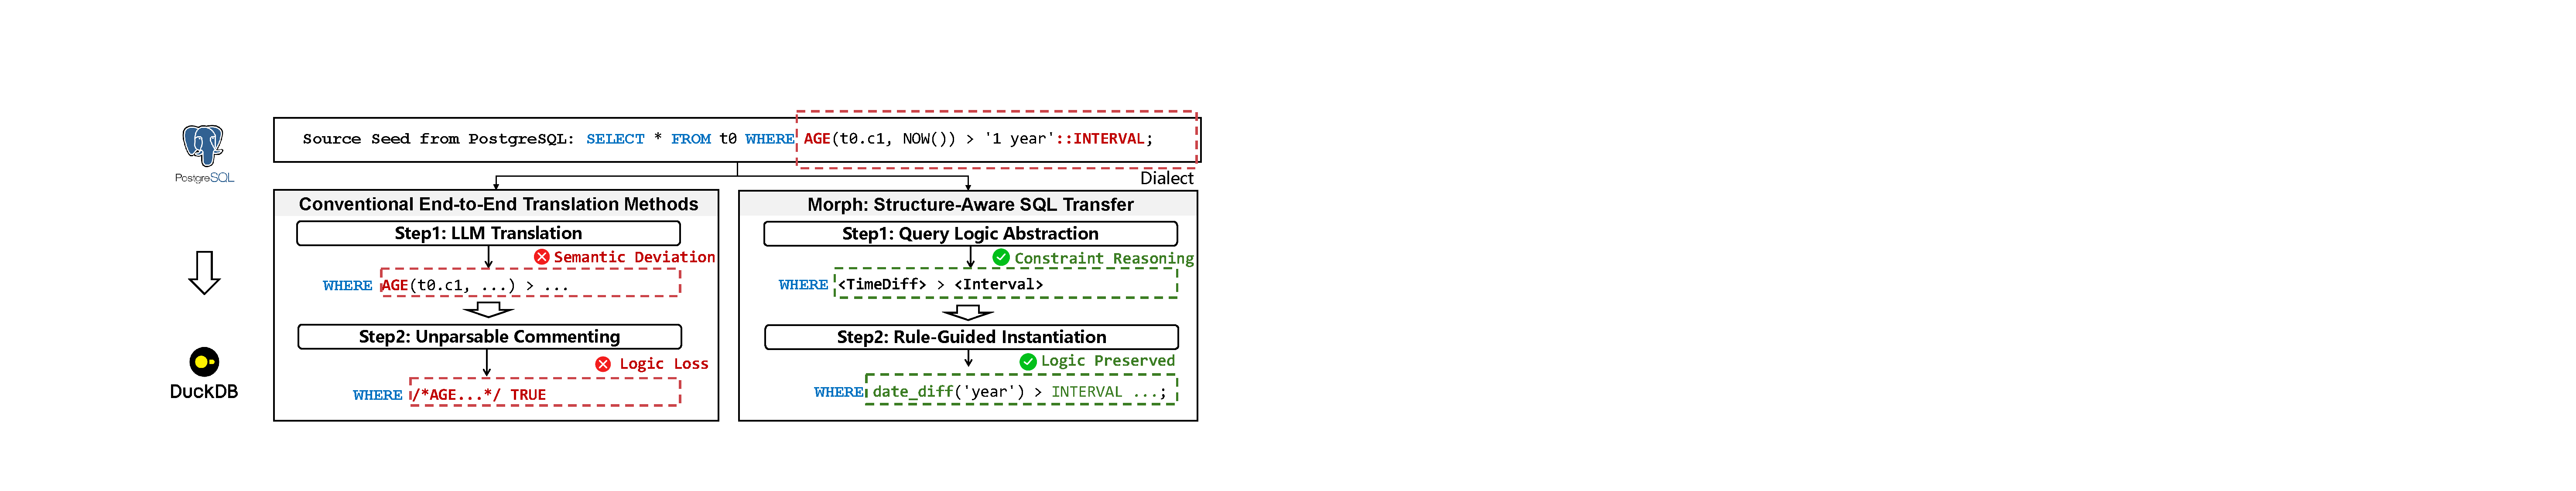
\includegraphics[scale=1.0, width=\linewidth]{media/motivating_new.pdf}
  \caption{Traditional end-to-end translation methods that directly convert seeds from \pg{} to \duckdb{} may introduce translation errors and logic loss.
  % The source query contains a dialect-specific function \texttt{AGE} and a type cast \texttt{::INTERVAL}. 
  Traditional Methods like \sedar{} suffer from \textit{hallucinations} (retaining \texttt{AGE}) and perform \textit{rigid sanitization} (removing the clause), resulting in a trivial query (Left). 
 \tool{} decouples intent via AQT, successfully instantiating the equivalent \texttt{date\_diff} logic (Right).}
 % \vspace{-1cm}
 % , thereby triggering deep execution paths 
  % \Description{A comparison diagram showing SQL query translation from PostgreSQL to DuckDB. The left side shows \sedar{}'s approach with semantic hallucinations and rigid sanitization, while the right side demonstrates Morph's \textit{Abstraction-then-Instantiation} approach preserving query semantics.}
  \label{fig:motivation}
\end{figure}


% \textbf{Limitations of Existing Approaches.} 
% Although LLM-based transfer methods have lowered the barrier for seed generation, they exhibit inherent limitations when handling strict SQL semantics. These limitations manifest primarily as \textit{semantic hallucinations} and \textit{logic loss}. 
% \textit{Semantic hallucinations} arise when LLMs fail to bridge dialect gaps. For instance, directly translating a source query containing the PostgreSQL-specific \texttt{AGE(timestamp)} often results in the retention of this function in the target DuckDB query. Since the target dialect does not support this operator, the generated seed becomes semantically invalid.
% More critically, current approaches often sacrifice semantic integrity for syntactic compliance, leading to \textit{logic loss}. When encountering unsupported syntax (e.g., PostgreSQL's \texttt{::INTERVAL}), tools like \sedar{}~\cite{fu2024sedar} typically prune the incompatible clauses to ensure parsability.

\textbf{Motivating Example.}
LLM-based cross-dialect transfer methods help in the generation of initial fuzzer seeds but may introduce \textit{semantic deviation} due to hallucinations. 
Moreover, many fuzzers cover only a subset of SQL grammar. 
Existing methods typically comment out unsupported features to support seed mutation after transfer, which alters the query and causes the \textit{logic loss}.

\textit{Limitations of Existing Approaches.} Figure \ref{fig:motivation} illustrates the semantic deviation and logic loss \sedar{} experiences when transferring a test case from \pg{} to \duckdb{}, which contains dialect-specific features like the \texttt{AGE} function in the \texttt{WHERE} clause and the \texttt{::INTERVAL} type cast. With limited knowledge of \duckdb{}’s syntax, the LLM hallucinates and preserves \texttt{AGE}, causing syntax and semantic errors. To satisfy parsing constraints, \sedar{} comments out \texttt{AGE} and replaces the \texttt{WHERE} condition with \texttt{True}, producing a syntactically valid but simplified query that loses the original verification intent and fails to exercise deep internal states. As a result, the migrated seed offers minimal utility for effective DBMS testing.

% Figure \ref{fig:motivation} illustrates the semantic deviation and logic loss encountered by \sedar{} when transferring a test case from \pg{} to \duckdb{}, which contains dialect-specific features such as the \texttt{AGE} function in the \texttt{WHERE} clause and the \texttt{::INTERVAL} type cast. 
% Because the LLM has limited knowledge of \duckdb{}’s syntax, it hallucinates and preserves the original \texttt{AGE} function, resulting in a syntax error and semantic deviation.
% Moreover, to ensure the query satisfies the parsing constraints of the target \duckdb{}, \sedar{} comments the \texttt{AGE} function and simply sets the condition after the \texttt{WHERE} clause to \texttt{True}. 
% This simplification results in a syntactically valid but structurally simplified query that lacks the original verification intent and consequently fails to reach deep internal states such as the node copying logic within the Binder layer.
% Consequently, the migrated seed retains minimal utility for effective DBMS testing.

% To ensure the query satisfies the parsing constraints of the target DuckDB engine, \sedar{} often removes complex nested structures or replaces the filtering clause with a trivial TRUE constant. 


% % \textbf{Semantic Hallucination and Logic Loss.} 
% When a source query contains the PostgreSQL-specific time function \texttt{AGE(timestamp)}, relying directly on end-to-end LLM translation often results in hallucinations where the function call is retained, despite DuckDB not supporting it. This renders the generated seed semantically invalid.

% %\textbf{Logic Loss.} 
% More critically, current approaches often prioritize syntactic compliance over semantic preservation. When encountering dialect-specific syntax that exceeds the target fuzzer's grammar support (e.g., the compact type cast \texttt{::INTERVAL} in PostgreSQL), tools like \sedar{}~\cite{fu2024sedar} typically remove the incompatible clauses to ensure the query is parsable. While this strategy improves the syntactic pass rate, it inadvertently discards critical test logic. As shown in Figure~\ref{fig:motivation}, removing the time-window constraint degrades a complex test case into a trivial query (e.g., \texttt{WHERE TRUE}), rendering it incapable of reaching the deep optimization paths it was originally designed to trigger~\cite{fu2024sedar}.

% --- 插入图片代码开始 ---
% \begin{figure}[h]
%   \centering
%   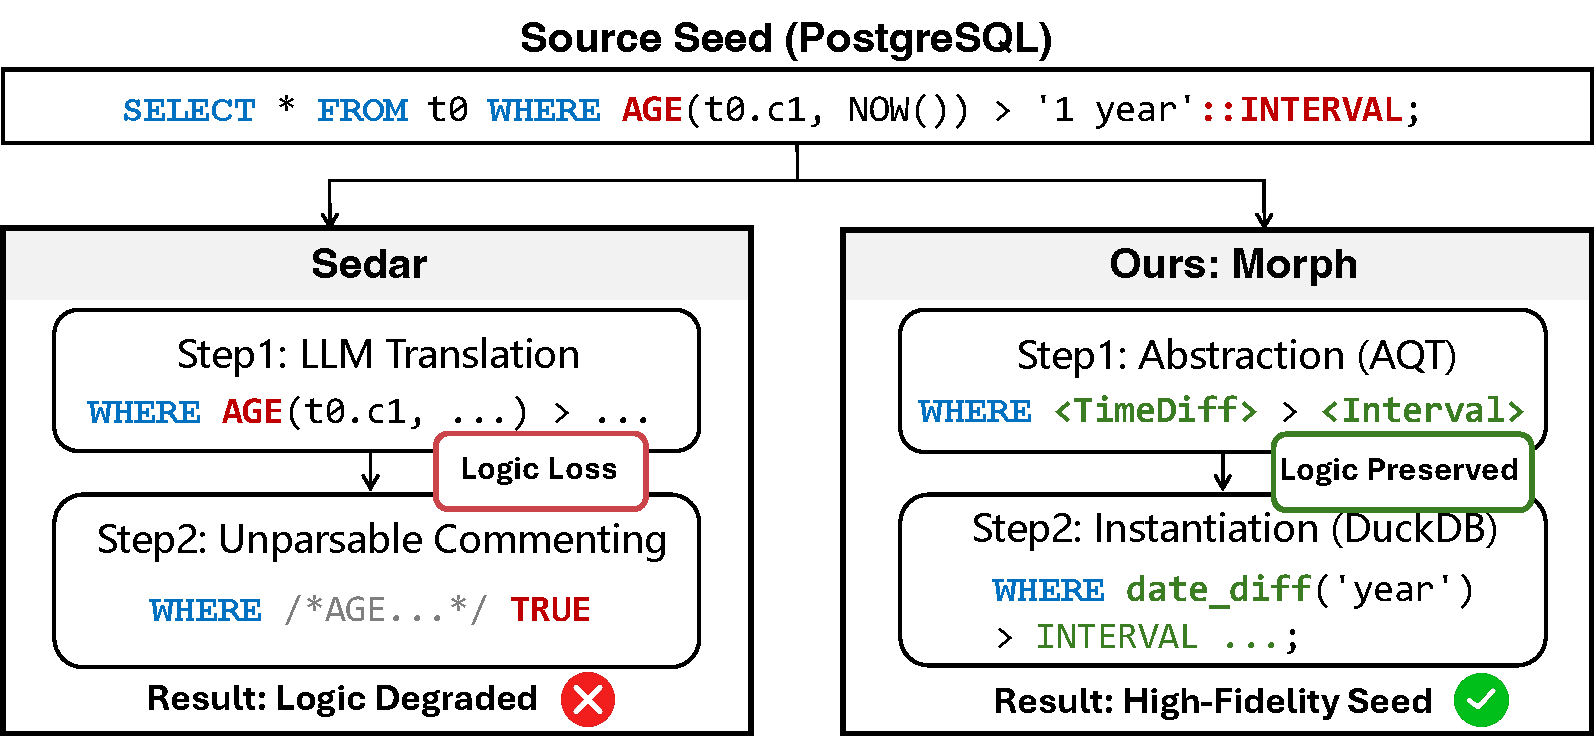
\includegraphics[width=\linewidth, height=7cm, keepaspectratio]{media/Motivation.pdf}
%   \caption{\textbf{Motivating Example: Transferring a seed from PostgreSQL to DuckDB.} 
%   The source query contains a dialect-specific function \texttt{AGE} and a type cast \texttt{::INTERVAL}. 
%   \textbf{(Left)} The baseline (\sedar{}~\cite{fu2024sedar}) suffers from \textit{hallucinations} (retaining \texttt{AGE}) and performs \textit{rigid sanitization} (removing the clause), resulting in a trivial query. 
%   \textbf{(Right)} \tool{} decouples intent via AQT, successfully instantiating the equivalent \texttt{date\_diff} logic, thereby triggering deep execution paths.}
%   \Description{A comparison diagram showing SQL query translation from PostgreSQL to DuckDB. The left side shows \sedar{}'s approach with semantic hallucinations and rigid sanitization, while the right side demonstrates Morph's \textit{Abstraction-then-Instantiation} approach preserving query semantics.}
%   \label{fig:motivation}
% \end{figure}


% --- 插入图片代码结束 ---

% Taking the migration from PostgreSQL to DuckDB as a running example (as illustrated in Figure~\ref{fig:motivation}):






\textit{Basic Idea of \tool{}.}
% To address the hallucinations and logic loss inherent in existing cross-dialect transfer methods, 
The core idea of \tool{} is to thoroughly decouple logical intent from syntactic representation, shifting from unstable textual translation to more robust structural recursive substitution. 
% \tool{} implements an \textit{Abstraction-then-Instantiation} paradigm that utilizes static analysis to extract dialect-agnostic Abstract Query Templates (AQT) preserving logical topology, and subsequently employs a rule-guided recursive substitution strategy to accurately map these templates to the target dialect for robust and non-destructive logic adaptation.
% We find that decoupling invariant query structure and semantics from dialect-specific syntax facilitates cross-dialect SQL transfer, rather than directly translating SQL text across DBMSs.
% Key challenges in achieving this include extracting query logic, preserving semantics in translation, and adapting queries for fuzzers.
% Based on this core idea, \tool{} overcomes the limitation of \sedar{} by decoupling the user's intent from the specific dialect's syntax via the AQT mechanism. 
As shown in Figure~\ref{fig:motivation}, \tool{} does not perform erroneous syntactic translation,
% instead of pruning incompatible parts, \tool{} 
but instead abstracts the dialect-specific \texttt{AGE} function into a generic <TimeDiff> intent. 
It then performs a high-fidelity instantiation into \duckdb{}’s equivalent syntax. By ensuring the type casting and window function partition logic are preserved, \tool{} generates a high-fidelity seed that retains the original filtering complexity. 
% \tool{} triggers deep execution paths in the target DBMS, enabling the detection of intricate logic bugs that are otherwise unreachable.
By maintaining these complex semantics during transfer, \tool{} ensures the generated seeds are effective for validation, enabling them to reach deeper code paths within the database and uncover intricate logic bugs unreachable by \sedar{}.
% 正因为\tool{}在transfer的过程中保留了这种复杂的语义，这个种子才能有效的用于测试，因此能测试数据库更深层的代码路径，从而测试到了sedar测不到的bug（ID：XXX）

% Introduce overall workflow/architecture (with an overview figure)
% Describe procedures/subcomponents (with figures or algorithms or examples)
\section{Approach}
\label{sec:approach}



% \subsection{System Overview}
\tool{} is an automated cross-dialect DBMS fuzzing framework designed to transform high-quality test cases from a mature source DBMS into effective seeds for a target DBMS. 
%输出是bug这个表述有点奇怪
% The system takes raw SQL queries from the source DBMS as \textbf{Input} and outputs exposed vulnerabilities (e.g., crashes or logic bugs) in the target DBMS as \textbf{Output}.
As illustrated in Figure~\ref{fig:workflow}, \tool{} takes the original queries from the source database as input, leverages cross-dialect transform to generate high-quality test cases for the target database, and employs these test cases for vulnerability discovery.

\begin{figure*}[htbp]
  \centering
  
\includegraphics[width=\linewidth]{media/overview-new.pdf}
  \caption{\textbf{Overview of the \tool{}.} \tool{} generate high-quality cross-dialect test cases following three steps: 
  (1) Syntax-Aware Query Abstraction. \tool{} first parses SQL into an AST and extracts schema information.  Then it replaces dialect-specific syntax with generic labels to build AQTs.
  (2) Rule-Guided Recursive Dialect Instantiation. \tool{} uses a task planner to decompose complex test case transformations and a hybrid knowledge base to guide the LLM, enabling SQL transformation, rule generation, and error correction.
  (3) Feedback-Driven Adaptive Fuzzing. \tool{} adapts fuzzer-incompatible test cases using runtime feedback, preserving core logic while ensuring parsability and maximal coverage.}
  \label{fig:workflow}
  \vspace{-0.5cm}
\end{figure*}

% As illustrated in Figure~\ref{fig:workflow}, the workflow of \tool{} operates as a closed loop following the \textit{Abstraction-then-Instantiation} paradigm, consisting of three cascaded stages:

% --- 插入跨双栏的工作流图 ---

  % Morph recursively replaces AQT nodes with dialect-specific subtrees using rules from a Hybrid Knowledge Base, which is continuously updated during translation. Each node first checks for an existing rule in the knowledge base. If one exists, it is mapped to an equivalent subtree; If not, a new rule is generated using LLMs and added to the knowledge base
  % \tool{} leverages a task planner to decompose complex test case transformation tasks into a sequence of statement translation tasks. In addition, \tool{} constructs a hybrid knowledge base to provide the LLM with relevant syntactic and grammatical rules, thereby ultimately enabling the RAG agent to perform SQL transformation, rule generation, and error correction.
  % \tool{} modifies test cases that are incompatible with the fuzzer, guided by runtime feedback. Test cases are modified into parsable forms while perserving deep logical structures, ensuring maximal testing coverage and bug detection
  %感觉有点多了，可以精简描述
  % \Description{A workflow diagram illustrating Morph's three-phase architecture: Syntax-Aware Query Abstraction extracts AQTs from source SQL, Rule-Guided Recursive Instantiation generates target-compatible seeds using an LLM agent, and Feedback-Driven Adaptive Sanitization refines seeds based on fuzzer feedback.}
 
% -------------------------AQT的概念在intro中提出过吗？
% \begin{enumerate}
%     \item \textbf{Syntax-Aware Query Abstraction:} 
%     The process begins with the static analysis engine receiving source SQL test cases. By leveraging schema information and AST parsing techniques, the engine strips away dialect-specific syntax details (e.g., type modifiers or specific function names). It extracts \textit{AQT} that preserve the core logical skeleton, such as query topology and data flow dependencies. This stage effectively achieves the decoupling of logical intent from syntactic representation.

%     \item \textbf{Rule-Guided Dialect Translation:} 
%     As shown in the middle panel of Figure~\ref{fig:workflow}, the extracted AQT are fed into the translation engine. A \textit{Task Planner} decomposes the complex instantiation task and coordinates a \textit{Hybrid Knowledge Base} with \textit{Test-Oriented Skill Execution}. Through the collaborative execution of sub-skills, specifically the \textit{SQL Translator}, \textit{Rule Generator}, and \textit{Error Fixer}, the engine recursively instantiates abstract nodes into concrete target dialect syntax, generating syntactically \textit{Compatible Seeds}.

%     \item \textbf{Feedback-Driven Mutation Loop:} 
%     In the final stage, the compatible seeds enter the fuzzing loop (right panel of Figure~\ref{fig:workflow}). An \textit{Adaptive Query Sanitizer} interacts with the downstream DBMS Fuzzers (e.g., Squirrel\cite{zhong2020squirrel} or Griffin~\cite{fu2022griffin}). Instead of destructively removing unparsable tokens, it adapts the seeds into \textit{Mutable Seeds} that are strictly parsable by the fuzzer's internal grammar. These seeds are then continuously mutated and executed, ultimately triggering hidden \textbf{BUGS} in the target system.
% \end{enumerate}

% In the following paragraphs, we elaborate on the design details of three stages.

\subsection{Syntax-Aware Query Abstraction}
\label{sec:abstraction}

The primary objective of this stage is to extract generic logic by decoupling the \textit{logical intent} of a test case from its \textit{dialect-specific representation}. 
The challenge is extracting generic query logic from tightly-coupled dialects.
We formalize the seed structure to extract generic logic and enable precise manipulation.
For better understanding, we first give some formal definition of basic concepts.




% 定义定理环境
\numberwithin{equation}{section} % 公式按章节编号（可选）
% \newtheorem{definition}{Definition}[section] % Definition 按 section 编号

\subsubsection{Formal Definition}
To support syntax-aware query abstraction and decouple the logical intent of a test case, we introduce the SQL abstraction rules and AQT. 
% A abstraction rule mappings from one dialect-specific construct to abstract representations to support cross-dialect translation.
They are defined as follows:
\vspace{-0.5cm}
\begin{list}{}{\setlength{\leftmargin}{0.5em}}
\item
    \begin{definition}[SQL Abstraction Rule]\label{def:rules}
    Abstraction rules map from one dialect-specific construct to abstract representations. A rule has the form:
    % $\text{source} \;\rightarrow\; \text{target}$, 
    \[
        Source: [Funtion | Type | ...] \rightarrow Target: [<FuncTag> | <TypeCast> | ...]
    \]
    where \textit{Source} is a dialect-specific SQL element and \textit{Target} is its corresponding abstract label that represents the semantic intent. For example, a rule from \pg{} to \duckdb{} can be represent as $\texttt{AGE}(\cdot) \;\rightarrow\; \langle \text{TimeDiff} \rangle$.
    
    % \textit{Source}: [\texttt{AGE}($\cdot$) $|$ \texttt{::INT} $|$ \texttt{MIN}($\cdot$)] $\rightarrow$ \textit{Target}: [$\langle$\texttt{TimeDiff}$\rangle$ $|$ $\langle$\texttt{TypeCast}$\rangle$ $|$ $\langle$\texttt{AggMin}$\rangle$].
    % For example, the set $R$ may include:
    % \[
    % \texttt{AGE}(\cdot) \;\rightarrow\; \langle \text{TimeDiff} \rangle, \quad
    % \texttt{::INT} \;\rightarrow\; \langle \text{TypeCast} \rangle, \quad
    % \texttt{MIN}(\cdot) \;\rightarrow\; \langle \text{AggMin} \rangle.
    % \]
    % These rules systematically replace dialect-specific syntax with abstract placeholders while preserving the semantic intent of the original query.
    \end{definition}


\item
    \vspace{-0.5cm}
    \begin{definition} [Abstract Query Template] \label{def:aqt}
    An AQT is defined as a 5-tuple:
    $$\mathcal{T} = \langle S_{norm}, \mathcal{D}, \mathcal{G}, \mathcal{C}, H  \rangle$$
    \begin{itemize}
        \item $S_{norm}$ denotes a \textit{Normalized SQL Skeleton} that masks dialect-specific literals and identifiers with abstract placeholders while preserving standard SQL keywords.
        \item $\mathcal{D}$ represents the \textit{Schema Context}, containing table and column definitions required.
        % to validate the query.
        \item $\mathcal{G} = (V, E)$ is the \textit{Structure Graph}, a directed acyclic graph where nodes $V$ represent logical segments (e.g., main statement, subqueries) and edges $E$ represent nesting dependencies. % (as shown in Figure~\ref{fig:aqt_trans}).
        \item $\mathcal{C}$ is the \textit{Complexity Score}, a weighted metric derived from AST depth, join count, and segment count, used to prioritize seeds during fuzzing scheduling.
        \item $H$ is a unique identifier for deduplication in RAG retrieval, calculated by hash function.  
        % the \textit{Structural Hash Fingerprint}, computed as $\mathcal{H} = \text{SHA256}(\|_{i \in V} S_{norm}^{(i)})$. It serves as a unique identifier for deduplication in our RAG retrieval.
        
    \end{itemize}
    \end{definition}

\end{list}



% add 超链接标号
\subsubsection{Semantic-Aware Abstraction Process}%+algorithm display + real case
% The abstraction process transforms a concrete SQL query into this structured tuple. To extract high-level structural semantics while abstracting away dialect-specific details, \tool{} generates the AQT five-tuple using Algorithm~\ref{alg:aqt_extraction}. Specifically, \tool{} first parses the source query $Q_{src}$ into a schema-bound AST (Line~\ref{line:alg1:parse}). It then performs a recursive decomposition via the \textsc{Traverse} function (Lines~\ref{line:alg1:traverse_start}--\ref{line:alg1:traverse_end}), which identifies logical boundaries (Lines~\ref{line:alg1:boundary_start}--\ref{line:alg1:boundary_end}) and applies abstraction rules $\mathcal{R}$ to simplify complex expressions (Lines~\ref{line:alg1:rule_start}--\ref{line:alg1:rule_end}), while preserving standard tokens otherwise (Line~\ref{line:alg1:else}). During this traversal, \tool{} constructs a structural graph $\mathcal{G}$ to capture nesting dependencies (Line~\ref{line:alg1:addedge}) and stores the resulting query segments in $Segs$ (Line~\ref{line:alg1:segs}). Finally, \tool{} computes a normalized skeleton $S_{norm}$, a structural hash $\mathcal{H}$, a complexity score $\mathcal{C}$, and the schema context $\mathcal{D}$ to assemble the complete AQT (Lines~\ref{line:alg1:norm}--\ref{line:alg1:return}). This structured representation allows \tool{} to treat queries as manipulable graph objects rather than flat strings.

The abstraction process transforms a concrete SQL query into a structured AQT tuple using Algorithm~\ref{alg:aqt_extraction}. 
\tool{} first parses the source query $Q_{src}$ into a schema-bound AST (Line~\ref{line:alg1:parse}) and recursively decomposes it via the \textsc{Traverse} function (Lines~\ref{line:alg1:traverse_start}--\ref{line:alg1:traverse_end}), identifying logical boundaries (Lines~\ref{line:alg1:boundary_start}--\ref{line:alg1:boundary_end}) and applying abstraction rules $\mathcal{R}$ (Lines~\ref{line:alg1:rule_start}--\ref{line:alg1:rule_end}) while preserving standard tokens otherwise (Line~\ref{line:alg1:else}). During traversal, a structural graph $\mathcal{G}$ captures nesting dependencies (Line~\ref{line:alg1:addedge}) and query segments are stored in $Segs$ (Line~\ref{line:alg1:segs}). Finally, \tool{} computes a normalized skeleton $S_{norm}$, a structural hash $\mathcal{H}$, a complexity score $\mathcal{C}$, and the schema context $\mathcal{D}$ to assemble the complete AQT (Lines~\ref{line:alg1:norm}--\ref{line:alg1:return}). This representation allows queries to be manipulated as structured graph objects rather than flat strings.


% ============================================================
% Algorithm 1: Structure-Aware AQT Generation (Compact)
% ============================================================
% \vspace{-0.5cm}
\begin{algorithm}[ht]
\small
\caption{Structure-Aware AQT Generation}
\label{alg:aqt_extraction}

\SetKwInOut{Input}{Input}
\SetKwInOut{Output}{Output}
\SetKwProg{Fn}{Function}{:}{}

\Input{Source query $Q_{src}$; Schema $\mathcal{S}$; Abstraction rules $\mathcal{R}$}
\Output{AQT $\mathcal{T} = \langle S_{norm}, \mathcal{D}, \mathcal{G}, \mathcal{H}, \mathcal{C} \rangle$}

$\mathcal{G} \leftarrow \emptyset$; $Segs \leftarrow \emptyset$ \tcp*{Structure graph; segment storage}
$AST \leftarrow \textsc{Parse}(Q_{src}, \mathcal{S})$ \tcp*{Build AST with schema binding} \label{line:alg1:parse}
$root \leftarrow \textsc{Traverse}(AST.root, \textsc{Null})$ \tcp*{Recursive decomposition}
$S_{norm} \leftarrow \textsc{Normalize}(Segs[root])$ \tcp*{Normalized skeleton} \label{line:alg1:norm}
$\mathcal{H} \leftarrow \textsc{SHA256}(S_{norm})$; $\mathcal{C} \leftarrow \textsc{Complexity}(AST)$ \tcp*{Hash; score}
$\mathcal{D} \leftarrow \textsc{ExtractSchema}(\mathcal{S}, Q_{src})$ \tcp*{Schema context}
\Return $\langle S_{norm}, \mathcal{D}, \mathcal{G}, \mathcal{H}, \mathcal{C} \rangle$\; \label{line:alg1:return}

\hrulefill

\Fn{\textsc{Traverse}($node$, $pid$)}{ \label{line:alg1:traverse_start}
    $id \leftarrow \textsc{NewID}()$; $tokens \leftarrow [\,]$\;
    \lIf{$pid \neq \textsc{Null}$}{$\mathcal{G}.\textsc{AddEdge}(pid \to id)$} \label{line:alg1:addedge}
    \ForEach{$c$ \textbf{in} $node.children$}{
        \uIf{\textsc{IsBoundary}($c$)}{ \label{line:alg1:boundary_start}
            $cid \leftarrow \textsc{Traverse}(c, id)$ \tcp*{Recurse into subquery/CTE}
            $tokens.\textsc{Append}(\texttt{<SubQuery:}cid\texttt{>})$\; \label{line:alg1:boundary_end}
        }
        \uElseIf{$r \leftarrow \textsc{MatchRule}(c, \mathcal{R})$}{ \label{line:alg1:rule_start}
            $tokens.\textsc{Append}(r.abstract)$ \tcp*{e.g., AGE()$\to$<TimeDiff>} \label{line:alg1:rule_end}
        }
        \lElse{$tokens.\textsc{Append}(c.text)$} \label{line:alg1:else}
    }
    $Segs[id] \leftarrow tokens$; \Return $id$\; \label{line:alg1:segs}
} \label{line:alg1:traverse_end}
\end{algorithm}

\begin{figure}[b]
\centering
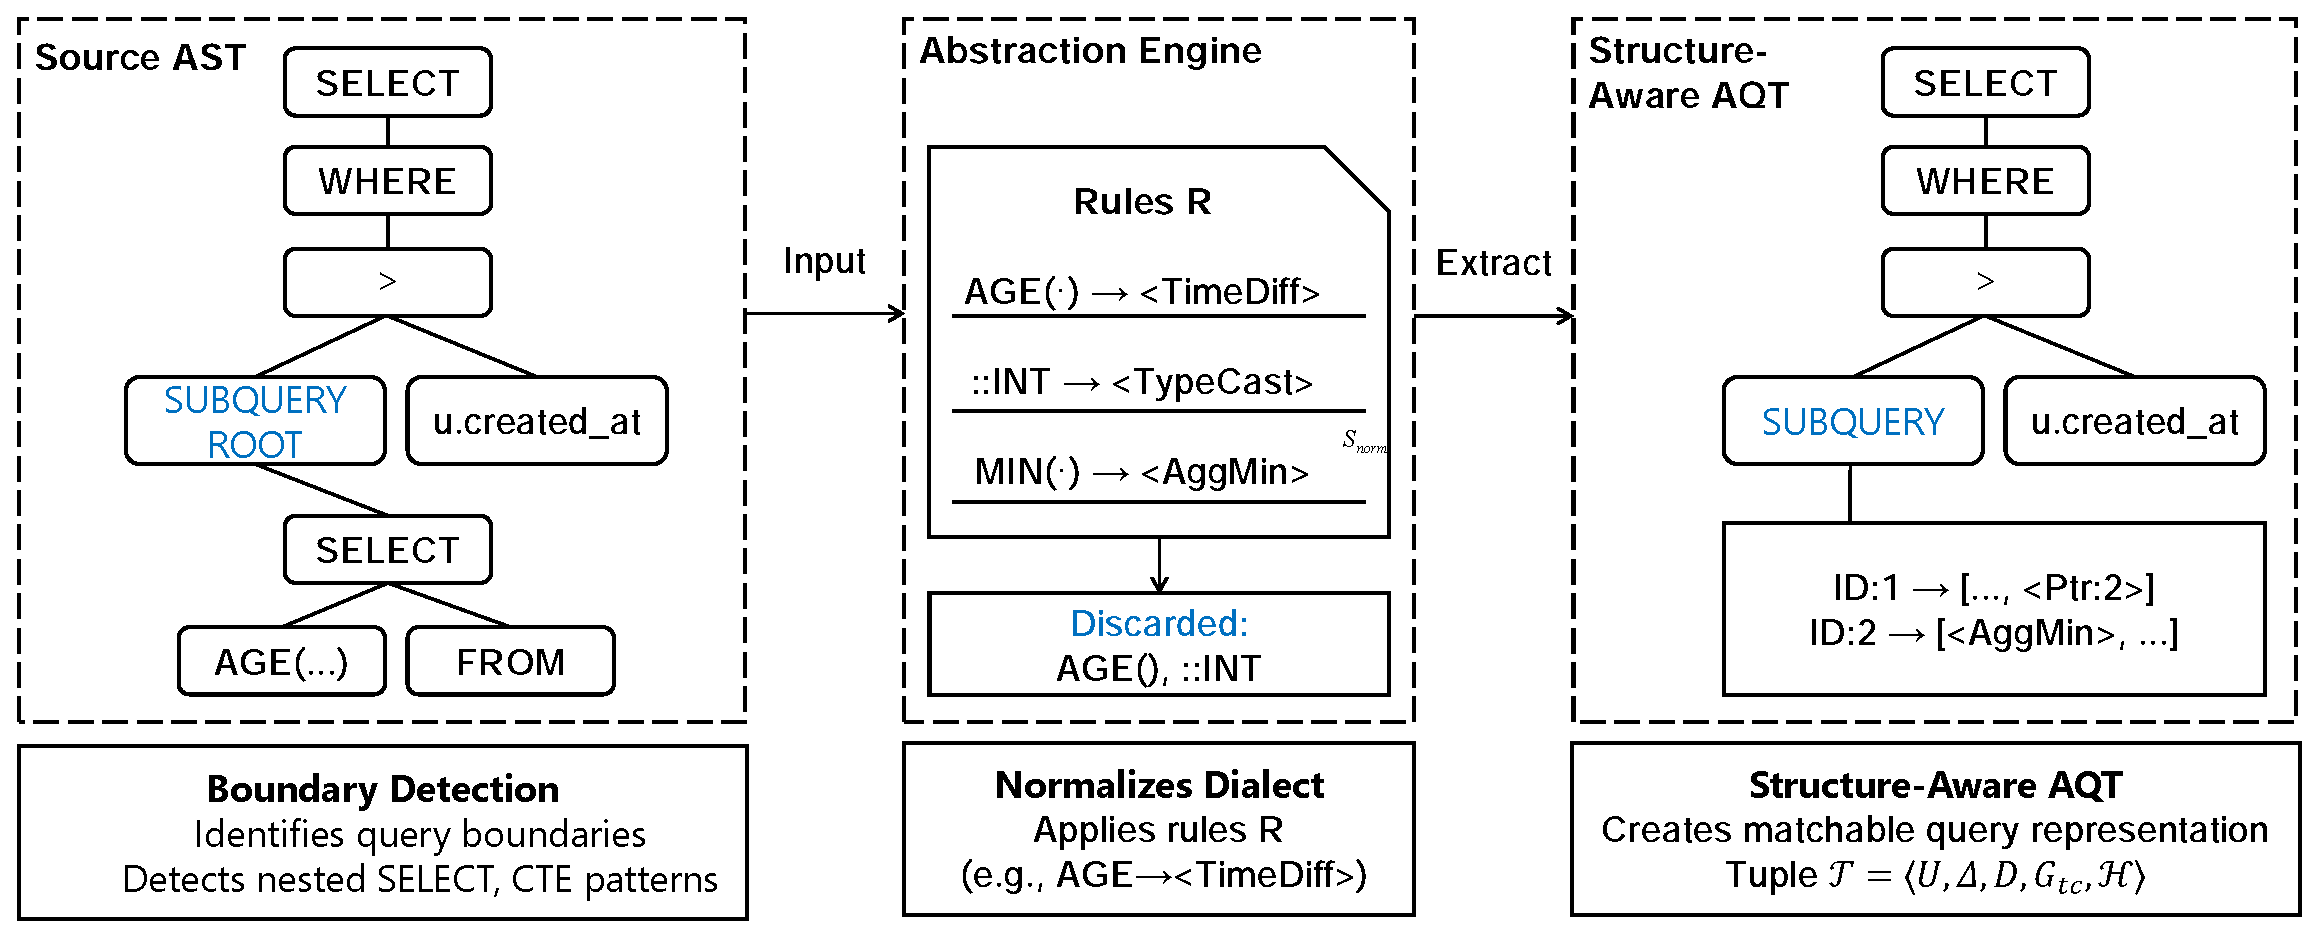
\includegraphics[scale=1.0, width=0.8\textwidth]{media/aqt.pdf}
    \caption{The Structure-Aware Abstraction Process. It first detects and normalize dialect-specific SQL features to abstract labels using abstraction rules, and producing structure-aware AQTs.}    
    % \cnum{1} \textbf{Detection:} Complex structures (red) trigger recursive splits. 
    % \cnum{2} \textbf{Normalization:} Dialect features are abstracted via rules (yellow). 
    % \cnum{3} \textbf{Result:} A normalized skeleton with pointers to extracted segments (green).}
    % \Description{A diagram showing the three-step abstraction process: detecting complex SQL structures, normalizing dialect-specific features using abstraction rules, and producing a normalized query skeleton with extracted segments.}
    \label{fig:aqt_trans}
\end{figure}

% \textbf{Example.}
To illustrate Algorithm~\ref{fig:aqt_trans}, Figure~\ref{fig:aqt_trans} presents a source SQL query with a nested subquery, where the outer query filters records using an age computation, for example ``\texttt{SELECT ... WHERE u.created\_at} > \texttt{(SELECT AGE(...) FROM ...)}''. The query is first parsed into an AST, and structural boundaries are identified during recursive traversal. 
The \texttt{SUBQUERY} ROOT node is detected as a boundary, decomposing the query into an outer block with ID 1 and an inner subquery with ID 2. The abstraction engine then applies rules $\mathcal{R}$ to normalize dialect specific constructs, abstracting \texttt{AGE(...)}, \texttt{::INT}, and \texttt{MIN(.)} into <TimeDiff>, <TypeCast>, and <AggMin>. 
Finally, a structure-aware AQT is constructed, capturing the parent-child relationship via a pointer <Ptr:2> and producing a normalized skeleton $S_{norm}$ that preserves logic while abstracting dialect differences.


\subsection{Rule-Guided Recursive Dialect Instantiation}
\label{sec:translation}
% To eliminate LLM semantic hallucinations during recursive substitution +challenge
% Dialect translation requires more than surface-level lexical substitution, as subtle semantic discrepancies across dialects including differences in operator behaviors and implicit type conversions can easily lead to misaligned query semantics. 
% To ensure that recursive subtree generation preserves the intended logical meaning, the system must strictly constrain the LLM’s output space during AQT construction, guaranteeing that each substituted subtree remains semantically consistent with the target dialect.
% Following the abstraction phase, the system obtains an AQT tuple. 
The primary objective of this step is to instantiate AQTs into a syntactically valid query that adheres to the target dialect's grammar while preserving the original logical intent.
The challenge is preserving semantic correctness in recursive SQL substitution.
% unlike fragile end to end textual translation, 
To address it, \tool{} transforms the instantiation task into a closed-loop reasoning process built on an RAG architecture. 
As illustrated in Figure~\ref{fig:agent_translation}, the process takes the AQTs as its input context and follows a three-stage pipeline. 
(i) First, the \textit{Task Planner} coordinates the execution flow according to structural dependencies. 
(ii) Second, \textit{Test-Oriented Skill Execution} synthesizes concrete SQL fragments by retrieving and incorporating relevant context from the hybrid KB, drawing on patterns similar to those in modern agent extension frameworks~\cite{anthropic-skills-2025}.
% synthesizes concrete SQL fragments with support from a hybrid knowledge base to enable precise context retrieval. 
(iii) Finally, \tool{} assembles these fragments into \textit{compatible seeds} and verifies their syntactic and semantic correctness.

\begin{figure}[htbp]
    \centering
    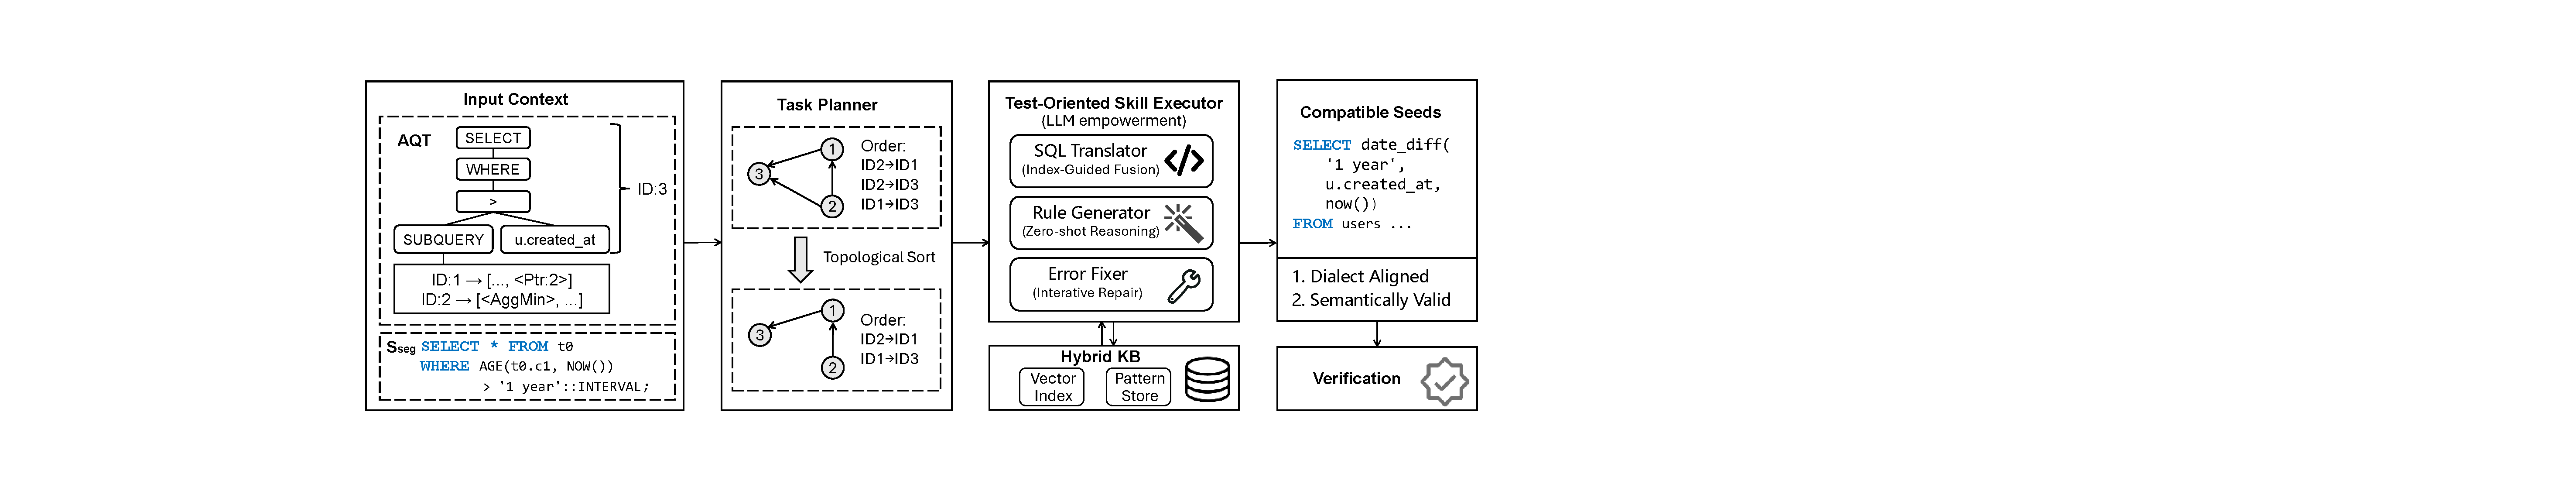
\includegraphics[scale=1.0, width=0.9\linewidth]{media/rule.pdf}
    \caption{\textbf{The RAG-enhanced Rule-Guided Translation Architecture.} 
    \cnum{1} \textit{Task Planning:} The Planner conducts a bottom-up topological sort on graph $\mathcal{G}$ to schedule the instantiation order. 
    \cnum{2} \textit{Knowledge-Augmented Execution:} The skill-execution method coordinates the Translator, Generator, and Fixer to instantiate abstract segments using context retrieved from the Hybrid KB. 
    \cnum{3} \textit{Seed Generation:} The system synthesizes \textit{Compatible Seeds} with guaranteed dialect alignment and semantic correctness.}
    \Description{An architecture diagram showing the RAG-enhanced translation system with three stages: task planning, knowledge-augmented skill execution using the hybrid KB, and seed generation producing compatible queries.}
    \vspace{-0.5cm}
    \label{fig:agent_translation}
\end{figure}


\subsubsection{Topological Task Planning}
The \textit{task planning} serves as the central orchestrator of the translation pipeline. Unlike naive line-by-line translation, \tool{} aims to resolve the complex variable scoping and nested dependencies inherent in SQL. To achieve this, the planner leverages the Structure Graph $\mathcal{G}$ to formulate a \textit{Bottom-Up Instantiation Strategy}, as illustrated in Figure~\ref{fig:agent_translation}.
Specifically, the planner treats each extracted segment $S_{seg}$ as a node in $\mathcal{G}$ and performs a \textit{topological sort} to derive an execution sequence $Order = \{id_1, id_2, \dots, id_n\}$. This ordering ensures a strict dependency resolution: independent leaf nodes, such as deeply nested subqueries or Common Table Expressions (CTEs), are instantiated and verified before their parent nodes. This modular approach prevents the context explosion problem in LLMs by ensuring that when a parent node is processed, its dependencies have already been reduced to concrete, dialect-compliant fragments.




\textit{Example.} In the scenario depicted in Figure~\ref{fig:agent_translation}, the planner identifies that the main query ($id_1$) depends on the aggregate result of a subquery (Segment $id_2$). Following the topological order $[id_2 \to id_1]$, the skill-execution method first instantiates Segment 2 to calculate the minimum timestamp. This fragment is then encapsulated and passed to the next stage as a known entity, allowing the planner to complete the outer query's construction without semantic ambiguity.

\subsubsection{Hybrid Knowledge Base}%+什么是hkb
To mitigate semantic hallucinations and drifts common in LLM-based code generation, \tool{} designs a \textit{Hybrid Knowledge Base} (Hybrid KB). As shown in Figure~\ref{fig:agent_translation}, this component provides grounded dialect constraints through two specialized storage engines:
% the bottom panel of 

\begin{itemize}
    \item \textbf{Abstract Pattern Store:} This storage maintains a repository of high-level SQL structural skeletons (e.g., specific \texttt{JOIN} topologies or \texttt{WINDOW} function templates). 
    By providing pre-validated patterns, the storage guides the LLM to preserve the \textit{syntactic topology}, keeping the query skeleton robust across dialect variants.
    % By providing these pre-validated patterns, the system guides the LLM to maintain the correct \textit{syntactic topology}, ensuring the skeleton of the generated query remains robust even for unconventional dialect variants.
    % Built upon a specialized vector database, 
    \item \textbf{Vector Index:} This storage stores fine-grained dialect knowledge, including official documentation, function signatures, and operator semantics. For any abstract token $\tau$ (e.g., \texttt{<TimeDiff>}), the system performs a semantic similarity search to retrieve the most relevant $k$ functional mappings. This retrieval-augmented approach transforms the translation task from ``creative generation'' to ``evidence-based instantiation.''
\end{itemize}


\subsubsection{Test-Oriented Skill Execution}%+LLM Skill 定义的解释
As shown in center panel of Figure~\ref{fig:agent_translation}, \textit{Test-Oriented Skill Execution} is the instantiation method that coordinates a suite of specialized skills under target-dialect constraints.



\begin{itemize}
    \item \textbf{SQL Translator:} The primary skill responsible for token-to-dialect mapping. It synthesizes the target SQL fragment by fusing the input segment with the function signatures retrieved from the \textit{Vector Index}. For instance, when encountering \texttt{<TimeDiff>}, it utilizes the retrieved \duckdb{} \texttt{date\_diff} signature to produce the final compliant expression.
    
    \item \textbf{Rule Generator:} This skill is triggered when the retrieval confidence for a specific feature falls below a threshold. It leverages the LLM's zero-shot reasoning to synthesize a new transformation rule based on the AST context and few-shot examples, which is then cached back into the \texttt{Hybrid KB} to refine the system's knowledge over time.
    
    \item \textbf{Error Fixer:} Functioning as a runtime monitor, this skill performs an immediate syntax check on the generated fragment using the target database's parser. If an error is detected, the fixer analyzes the compiler's feedback to iteratively repair the code, ensuring the final output is a \textit{Compatible Seed} with guaranteed execution.
\end{itemize}



To guarantee that the generated queries remain semantically consistent with the target dialect during recursive construction, \tool{} employs a rule-guided instantiation process as formalized in Algorithm~\ref{alg:translation}. 
The algorithm first performs a topological sort on the structure graph $\mathcal{G}$ to determine a bottom-up execution sequence (Line~\ref{line:alg2:sort}), ensuring nested subqueries are resolved before their parents. For each segment, the planner recursively substitutes instantiated child fragments (Lines~\ref{line:alg2:substitute_start}). Each abstract token $\tau$ is instantiated using rules retrieved from the \texttt{Hybrid KB} (Line~\ref{line:alg2:retrieve}), or, if confidence is low, a generator creates a new rule (Line~\ref{line:alg2:generate}). The token is translated into target-compliant syntax (Line~\ref{line:alg2:translate}) and iteratively parsed and fixed (Line~\ref{line:alg2:fix}). Compliant fragments are then cached and assembled into the final seed $Q_{target}$ (Lines~\ref{line:alg2:cache}--\ref{line:alg2:assemble}).

% The algorithm first conducts a topological sort on the structure graph $\mathcal{G}$ to determine a bottom-up execution sequence (Line~\ref{line:alg2:sort}), ensuring that nested subqueries are resolved before their parent segments. 
% For each segment, the planner recursively substitutes previously instantiated child fragments (Lines~\ref{line:alg2:substitute_start}--\ref{line:alg2:substitute_end}). 
% To handle each abstract token $\tau$, the agent retrieves specific dialect rules from the Hybrid Knowledge Base (Line~\ref{line:alg2:retrieve}); if the retrieval confidence is low, a specialized generator synthesizes a new transformation rule (Line~\ref{line:alg2:generate}). 
% The token is then instantiated into target-compliant syntax (Line~\ref{line:alg2:translate}) and undergoes an iterative parsing-fix loop to resolve any residual syntax errors (Line~\ref{line:alg2:fix}). 
% Finally, the compliant fragments are cached and assembled into the final seed $Q_{target}$ (Lines~\ref{line:alg2:cache}--\ref{line:alg2:assemble}).

% +算法描述或换成图来解释
% ============================================================
% Algorithm 2: Rule-Guided Dialect Translation (Compact)
% ============================================================
\begin{algorithm}[htbp]
\small
\caption{Rule-Guided Recursive Dialect Instantiation}
\label{alg:translation}

\SetKwInOut{Input}{Input}
\SetKwInOut{Output}{Output}

\Input{AQT $\mathcal{T} = \langle S_{norm}, \mathcal{D}, \mathcal{G}, \mathcal{H}, \mathcal{C} \rangle$; Target dialect $D_t$; Hybrid KB $HKB$; Threshold $\delta$}
\Output{Compatible seed $Q_{target}$}

$Order \leftarrow \textsc{TopologicalSort}(\mathcal{G})$; $Fragments \leftarrow \emptyset$ \label{line:alg2:sort} \tcp*{Bottom-up order}
\ForEach{$id$ \textbf{in} $Order$}{
    $S \leftarrow \textsc{GetSegment}(\mathcal{T}, id)$\;
    \ForEach{$c$ \textbf{in} $\mathcal{G}.children(id)$}{
        $S \leftarrow \textsc{Substitute}(S, c, Fragments[c])$ \label{line:alg2:substitute_start} \;
    } \label{line:alg2:substitute_end}
    \ForEach{$\tau$ \textbf{in} $\textsc{AbstractTokens}(S)$}{
        $(rule, conf) \leftarrow \textsc{Retrieve}(HKB, \tau, D_t)$ \label{line:alg2:retrieve} \tcp*{Query Hybrid KB}
        \If{$conf < \delta$}{
            $rule \leftarrow \textsc{Generator}(\tau, D_t)$ \label{line:alg2:generate} \;
            $HKB.\textsc{Cache}(\tau, rule)$\;
        }
        $frag \leftarrow \textsc{Translator}(\tau, rule, \mathcal{D})$ \label{line:alg2:translate} \tcp*{Instantiate token}
        \While{$err \leftarrow \textsc{Parse}(frag, D_t)$}{
            $frag \leftarrow \textsc{Fixer}(frag, err)$ \label{line:alg2:fix} \;
        }
        $S \leftarrow \textsc{Replace}(S, \tau, frag)$\;
    }
    $Fragments[id] \leftarrow S$ \label{line:alg2:cache} \tcp*{Cache result}
}
\Return $Fragments[\textsc{Root}(\mathcal{G})]$ \label{line:alg2:assemble} \tcp*{Assemble final seed}
\end{algorithm}



\subsection{Feedback-Driven Adaptive Fuzzing}%+挑战+例子
\label{sec:mutation_loop}
To support advanced DBMS features that exceed the grammar coverage of generic fuzzers, \tool{} enables a non-destructive adaptation process during runtime. 
The challenge is adapting advanced SQL features for grammar-limited fuzzers.
Instead of relying on offline destructive sanitization that deletes unsupported constructs and causes logic loss, \tool{} maintains a dynamic feedback loop with the fuzzer to continuously ensure seed parsability. 
% Through this interaction, \tool{} can automatically convert unparsable constructs into equivalent forms understandable by the fuzzer or apply valid encapsulation when necessary, thereby preserving the original test logic while remaining compatible with rigid fuzzer grammars.
To achieve this, \tool{} maintains a feedback-driven mutation loop that continuously interacts with the downstream fuzzer at runtime. Unlike prior approaches that perform seed generation as a one-off offline step, \tool{} iteratively leverages parsing and execution feedback to rewrite or encapsulate unsupported constructs into valid equivalents. 
This process consists of the following three main steps:
% is achieved through the collaboration of the 
%This loop ensures that generated seeds remain consistently parsable and logic-preserving throughout fuzzing.


% In this section, we detail the runtime interaction between \tool{} and the downstream fuzzer. Unlike prior approaches that treat seed generation as a one-off offline task, \tool{} maintains a dynamic feedback loop to ensure the continuous validity of generated seeds.





\textit{Adaptive Query Sanitizing. }
% The core step of the adaptive fuzzing is the Adaptive Query Sanitizer. 
When a transferred seed $Q_{target}$ is fed into the fuzzer, it may still contain subtle syntax incompatibilities that were not captured by the static translation phase. Instead of discarding these seeds or destructively commenting out the unparsable tokens (as done in \sedar{}~\cite{fu2024sedar}), the sanitizer captures the parser's error message.

\textit{Error-Guided Repairing.} When an error signal is received (e.g., ``Syntax Error at SELEC''), \tool{} identifies the corresponding node in the AQT and applies a set of \textit{Sanitization Rules}. If no rule matches, the LLM \textit{Error Fixer} skill is invoked~\cite{fan2023automated} to locally rewrite the problematic structure into a compliant form. For example, a rejected window function syntax may be transformed into a standard aggregation form when possible.

\textit{Mutable Seed Generation.} Once a seed passes the fuzzer's parser, it is designated as a \textit{Mutable Seed}. \tool{} then identifies data-dependent components, such as literals and predicates, and marks them as mutable regions. This directs the fuzzer's mutation engine to focus on logic-altering variations rather than the fixed syntactic skeleton, accelerating the discovery of deep logic bugs.

% \TODO{Check this paragraph. }
% 图5具体展示了这三个组件是如何协同运作来实现自适应fuzzing的。当输入Compatible Seeds时，\textit{Adaptive Query Sanitizer}分析并捕捉到Compatible Seeds中细微语法不兼容问题，并根据syntactic feedback对种子做清洗。比如，这个过程可以automatically removes the excess brackets around the \texttt{date\_diff} function to produce a syntactically valid Mutable Seed。经过清洗后得到了Mutable Seed，Morph会将其在数据库中执行。如果执行无误，便说明他可以参与后续的fuzz，由\textit{Mutable Seed Generation}引导fuzz变异。如果执行异常，则由\textit{Error-Guided Repair}收集异常信息，根据异常信息与目标数据库的semantic feedback对种子做修正，比如将wrap the \texttt{c\_time} column with the \texttt{toDateTime()} function。
% The resulting Final Seed is then marked with mutable regions, allowing the fuzzer to focus on logic-altering mutations rather than getting stuck on basic syntax or type errors, thereby accelerating the discovery of deep logic bugs.

\begin{figure}[htbp]
  \centering
  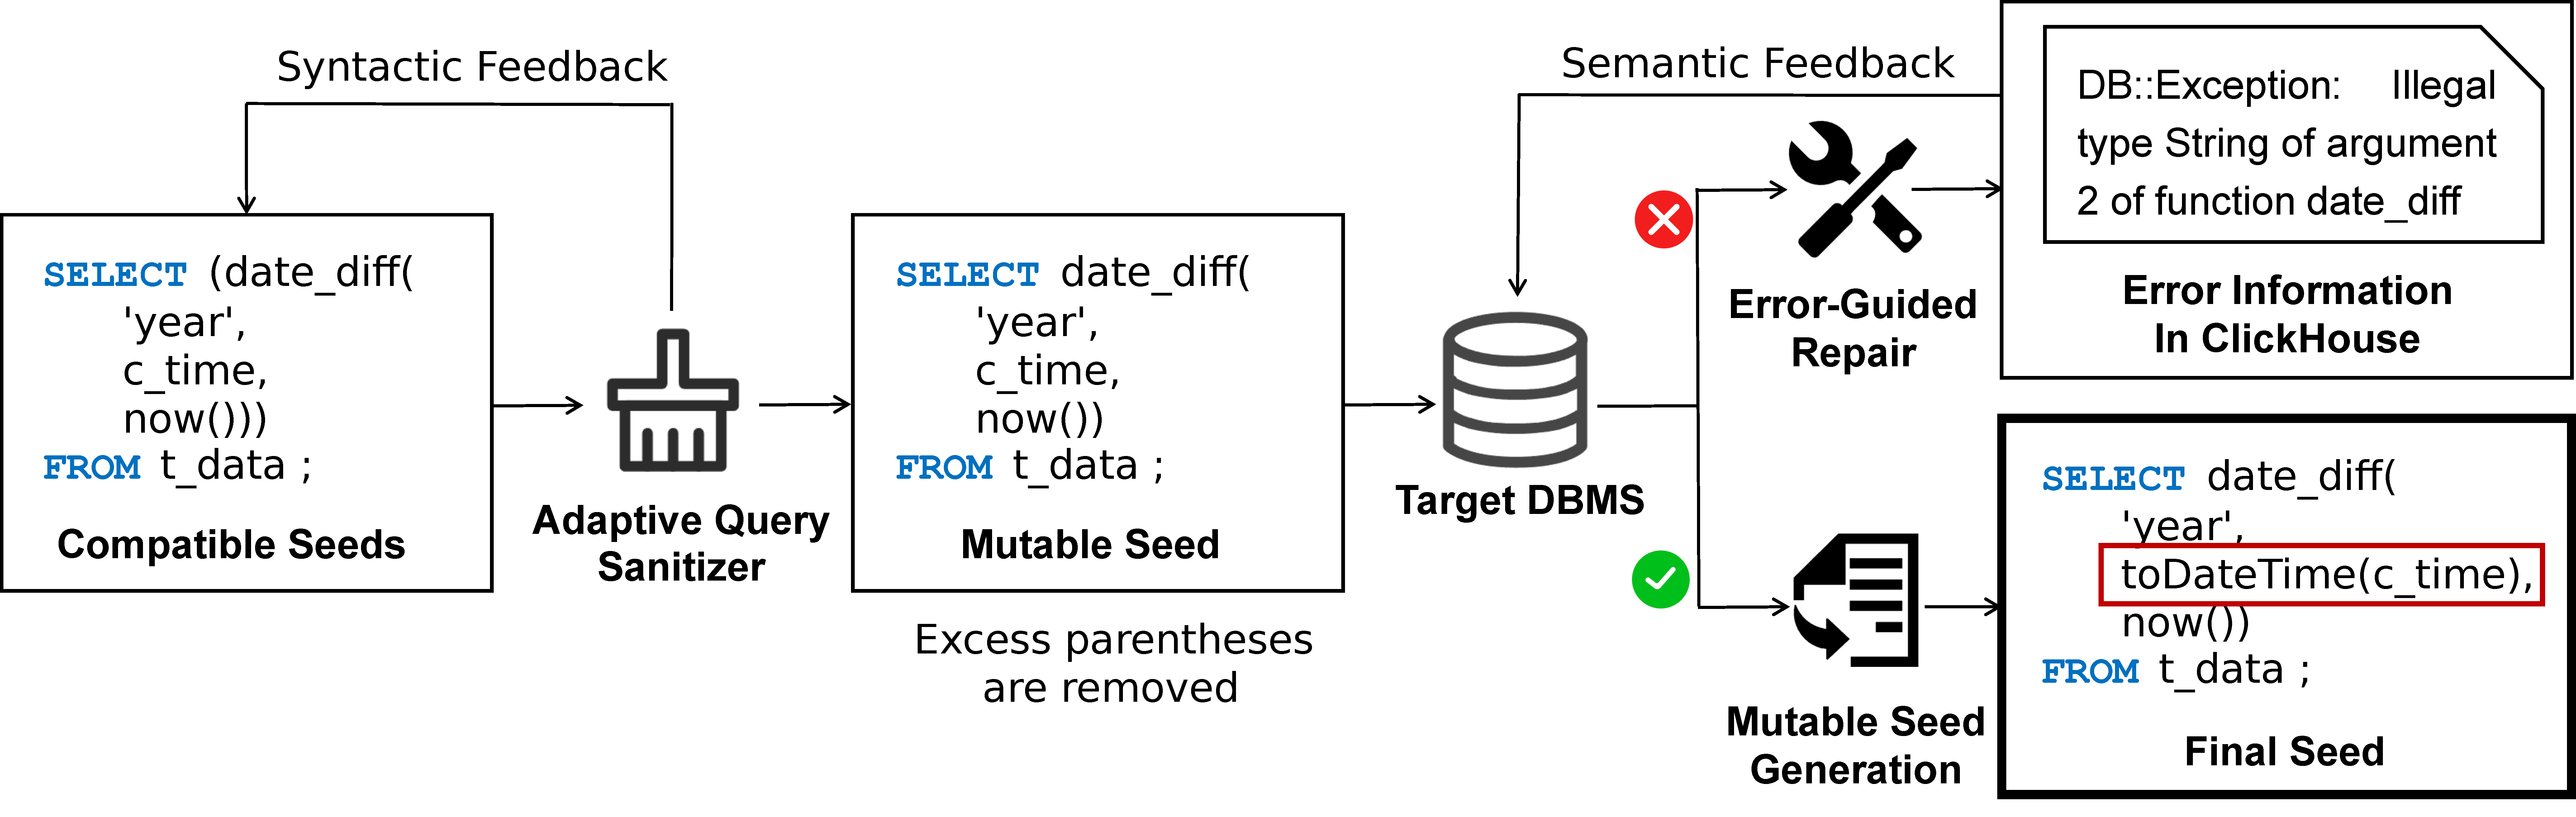
\includegraphics[scale=1.0, width=\linewidth]{media/feedback-driven.pdf}
  \caption{Collaborative Workflow of Adaptive Query Sanitizing, Error-Guided Repairing, and Mutable Seed Generation in Feedback-Driven Fuzzing.}
  \label{fig:feedback-driven}
\end{figure}

Figure~\ref{fig:feedback-driven} illustrates the collaborative workflow of these three components in achieving adaptive fuzzing. 
Upon receiving Compatible Seeds, the \textit{Adaptive Query Sanitizer} identifies subtle syntactic incompatibilities and cleans the seeds based on syntactic feedback. 
For instance, it automatically removes excess brackets around the \texttt{date\_diff} function to produce a syntactically valid Mutable Seed. \tool{} then executes this sanitized seed in the target database. If the execution succeeds, the \textit{Mutable Seed Generation} component immediately prepares the seed for subsequent fuzzing mutations. Conversely, if the execution fails, the \textit{Error-Guided Repair} component captures the error details and repairs the seed using semantic feedback, such as wrapping the \texttt{c\_time} column with the \texttt{toDateTime()} function. The resulting Final Seed is then marked with mutable regions, allowing the fuzzer to focus on logic-altering mutations rather than getting stuck on basic syntax or type errors, thereby accelerating the discovery of deep logic bugs.

\section{Evaluation}
\label{sec:evaluation}

\tool{} is implemented in Python and integrates \griffin{}~\cite{fu2022griffin}, a coverage-guided mutation fuzzer, as the downstream execution engine. For the LLM used in Test-Oriented Skill Execution and rule generation, we employ Gemini 2.5-flash-lite~\cite{gemini-2.5-flash} as the primary language model due to its strong code understanding capabilities and cost efficiency. We set the temperature parameter to 0.2 to balance determinism and output diversity, as justified by the sensitivity analysis discussion in Section~\ref{sec:llm-params}.
% Research questions
We evaluate \tool{} to assess its performance in cross-dialect seed transformation and its practical impact on DBMS fuzzing effectiveness. Specifically, our evaluation focuses on the following research questions:
\begin{itemize}
    \item \textbf{RQ1:} With \tool{} employed, can DBMS fuzzers find previously unknown vulnerabilities in production-grade DBMSs?
    \item \textbf{RQ2:} How does \tool{} compare to state-of-the-art baselines in terms of seed validity and preserving the semantic richness of source test cases?
    \item \textbf{RQ3:} Can transferred seeds improve the effectiveness of DBMS fuzzing?
    \item \textbf{RQ4:} How do the components of \tool{} contribute to the overall performance?
    % , including the \textit{Syntax-Aware Query Abstraction}, the \textit{Rule-Guided RAG Agent}, and the \textit{Feedback-Driven Adaptive Sanitizer}, 
\end{itemize}

    % \item \textbf{RQ4:} How do the individual components of \tool{}—specifically the \textit{Syntax-Aware Query Abstraction}, the \textit{Rule-Guided RAG Agent}, and the \textit{Feedback-Driven Adaptive Sanitizer}—contribute to the overall performance?
% Experiment setup (environment, benchmark, evaluation metrics, etc.)
\subsection{Experimental Setup}
\label{sec:setup}

% We detail the experimental environment, target systems, baselines, and metrics used to substantiate our evaluation.

\textbf{Target DBMSs and Environment.}
To evaluate the generalization of \tool{} across diverse architectures, we selected four widely used DBMSs according to the DB-Engines Ranking~\cite{dbengines}: MonetDB~\cite{monetdb} v11.51, Virtuoso~\cite{virtuoso} v7.2, DuckDB~\cite{duckdb_git} v1.1.3, and ClickHouse~\cite{clickhouse} v24.8 LTS. These systems span a broad spectrum of architectures, from embedded OLAP engines to distributed columnar stores, and while they share the relational data model, each implements a distinct SQL dialect.
% To evaluate the generalization of \tool{} across diverse architectures, we selected four popular DBMSs, including MonetDB~\cite{monetdb}, Virtuoso~\cite{virtuoso}, DuckDB~\cite{duckdb_git}, and ClickHouse~\cite{clickhouse}.
% These DBMSs are all widely used according to the DB-Engines Ranking~\cite{dbengines} and represent a broad spectrum of architectural designs, ranging from embedded OLAP systems to distributed columnar stores. While they share common relational data model features, they implement distinct SQL dialects. The specific versions under evaluation are MonetDB v11.51, Virtuoso v7.2, DuckDB v1.1.3, and ClickHouse v24.8 LTS.
% To evaluate generalization across diverse architectures, we selected four widely used DBMSs: MonetDB, a pioneer open-source column-store database; Virtuoso, a high-performance multi-model engine; DuckDB, an embedded in-process SQL OLAP system; and ClickHouse, a fast distributed columnar DBMS. We deployed the latest official Docker images for each to ensure a standardized environment: \TODO{MonetDB version1, Virtuoso version2, DuckDB verison3, ClickHouse verison4.}
We explicitly excluded traditional row-store OLTP systems (e.g., MySQL and PostgreSQL) from the target list, as they serve as the source DBMSs for seed collection. Instead, we prioritized OLAP and multi-model architectures to rigorously evaluate \tool{}'s capability in bridging significant dialectal and architectural gaps (i.e., from Row-store like \mysql{} to Column-store like \duckdb{}).
All experiments were conducted on a Linux server equipped with an Intel Xeon CPU and 256 GB of RAM. To ensure reproducibility and isolation, each DBMS instance ran within a separate Docker container.

\textbf{Collected Test Cases.}
Following the methodology of prior work~\cite{fu2024sedar}, we collected built-in test cases from mature DBMS repositories (i.e., SQLite~\cite{sqlite}, MySQL~\cite{mysql}, and PostgreSQL~\cite{pg}) as the source for transfer. Table~\ref{tab:collected_seeds} shows the statistics on collected test cases in each DBMS.
Specifically, the dataset aggregates 426,968 SQL statements across 6,695 files, totaling 54.4 MiB of query text. 

\begin{table}[h]
\centering
\caption{Statistics of collected open-source test cases from source DBMSs.}
\label{tab:collected_seeds}
\renewcommand\arraystretch{0.8}
\setlength{\tabcolsep}{6.5mm}{
    \scalebox{0.9}[0.9]{%
        \begin{tabular}{lccc}
            \toprule
            Source DBMS & Test Cases & Statements & Size \\
            \midrule
                SQLite & 2,643 & 308,292 & 31 MiB \\
                MySQL & 2,685 & 98,862 & 15 MiB \\
                PostgreSQL & 1,367 & 19,814 & 8.4 MiB \\
                \midrule
            Total & 6,695 & 426,968 & 54.4 MiB \\
            \bottomrule
        \end{tabular}
    }
}
\end{table}

\textbf{Baselines and Evaluation Metrics.}
We compare \tool{} against two distinct strategies, including No-Transfer and \sedar{}~\cite{fu2024sedar}. 
% serves as the lower bound for compatibility; it 
The No-Transfer (Raw Seeds) strategy involves directly executing the original test cases collected from source DBMSs without modification. 
\sedar{} represents the current state-of-the-art LLM-based transfer tool in constructing initial seeds in fuzzing. We faithfully reproduced \sedar{}'s complete pipeline, including schema capture, end-to-end LLM translation, and its comment-out sanitization strategy for evaluation.
% to evaluate \tool{} against the best existing solution.

We employ three comprehensive sets of metrics to evaluate \tool{}.
First, to assess transfer quality, we measure \textit{Syntactic Correctness} (the proportion of seeds passing the parser) and \textit{Semantic Validity} (the proportion executing without runtime errors). 
Second, to quantify the effectiveness in improving fuzzing, we utilize LLVM's \texttt{SanitizerCoverage} to track \textit{Branch Coverage} over 24-hour campaigns. We report the average results across five independent runs to mitigate randomness. 
Third, regarding real-world bug discovery, we present the detected number of bugs. 
The bugs are deduplicated from raw crash logs using stack hashes and error signatures, ensuring that the reported numbers reflect unique vulnerabilities.

% We compare \tool{} against two distinct strategies. First, Raw Seeds (No-Transfer) involves the direct execution of original test cases collected from source DBMSs (PostgreSQL, MySQL, SQLite) without modification, representing the lower bound of compatibility. Second, we compare against \sedar{}~\cite{fu2024sedar} (SOTA), the current state-of-the-art LLM-based transfer tool. We faithfully reproduced \sedar{}'s complete pipeline, including schema capture, end-to-end LLM translation, and its comment-out sanitization strategy.





% By leveraging these test suites from mature row-store engines , we ensure that the source seeds possess both syntactic correctness and logical depth, serving as a solid foundation for evaluation.
% These test cases encompass diverse SQL features including complex joins, window functions, and recursive CTEs, providing rich input diversity for seed generation.


% \paragraph{\textbf{Evaluation Metrics}}
% \lqf{
% We employ three comprehensive sets of metrics to evaluate \tool{}
% First, to assess transfer quality, we measure \textit{Syntactic Correctness} (the proportion of seeds passing the parser) and \textit{Semantic Validity} (the proportion executing without runtime errors). Second, to quantify deep logic exploration, we utilize LLVM's \texttt{SanitizerCoverage} to track \textit{Branch Coverage} over 24-hour campaigns. We report the average results across five independent runs to mitigate randomness. Third, to demonstrate practical effectiveness, we report the number of \textit{Unique Crashes} (deduplicated by stack trace) and \textit{Logic Bugs} discovered.
% }
% We employ three sets of metrics. First, validity statistics measure Syntactic Correctness (proportion of seeds passing the parser) and Semantic Validity (proportion of seeds executing without runtime errors), serving as the primary indicators of transfer quality. Second, regarding code coverage, we utilize LLVM's \texttt{SanitizerCoverage} to capture Branch Coverage over a 24-hour campaign. To mitigate randomness, we repeated each campaign 5 times and reported the average results to quantify deep logic exploration. Third, for bug discovery, we report the number of Unique Crashes (deduplicated by stack trace) and Logic Bugs detected.


% , and each fuzzing session was configured for a duration of 24 hours.


% Experimental results (answer the RQs one by one)
% \subsection{Experimental Results}
% \label{sec:results}

% In this section, we present the experimental results to answer our research questions. 
% Table~\ref{tab:validity} and Table~\ref{tab:diversity} summarize the comparative performance of \tool{} ($S^+$) against the raw seeds ($S^-$) and \sedar{} ($S$).

%============================================================
% Table: Real-World Bug Detection (单栏缩放 + 匿名化 + 精简描述)
% ============================================================
\begin{table}[b]
\centering
\caption{Statistics of previously unknown bugs in production-grade DBMSs detected with fuzzing with translated initial seeds by \tool{}. (Parts of the bug IDs have been replaced with ``XX'' for double-blind review.)}
\label{tab:real-world-bugs}
% \resizebox{\columnwidth}{!}{%
    \renewcommand\arraystretch{1}
    \setlength{\tabcolsep}{1mm}{
        \scalebox{0.95}[0.95]{%
            \begin{tabular}{cccccc}
            \toprule
            \textbf{\#} & \textbf{DBMS} & \textbf{Bug ID} & \textbf{Status} & \textbf{Component} & \textbf{Description} \\ \midrule
                1 & MonetDB & \#77xx & Reported & Optimizer & Incorrect boolean logic evaluation. \\
                2 & MonetDB & \#77xx & Fixed & Server & Failure during large data ingestion. \\
                3 & MonetDB & \#77xx & Reported & Server & Metadata corruption via system truncate. \\
                4 & MonetDB & \#77xx & Confirmed & Server & Irrecoverable catalog corruption. \\
                5 & MonetDB & \#78xx & Reported & Server & Crash in nested recursive set operations. \\
                6 & MonetDB & \#78xx & Reported & Server & Crash during dead code elimination. \\ 
                7 & Virtuoso & \#13xx & Confirmed & Server & Memory violation in ORDER BY. \\
                8 & Virtuoso & \#13xx & Confirmed & Server & SIGSEGV in HAVING clause functions. \\
                9 & DuckDB & \#201xx & Reported & Function & OOM triggered by abnormal padding. \\
                10 & DuckDB & \#205xx & Fixed & Executor & Internal error from type mismatch. \\
                11 & DuckDB & \#203xx & Confirmed & Binder & Node copy failure in window functions. \\
                12 & DuckDB & \#203xx & Reported & Executor & Floating point exception in CTEs. \\
                13 & ClickHouse & \#950xx & Confirmed & Function & SIGSEGV during result deserialization. \\
                14 & ClickHouse & \#951xx & Reported & Server & Mutation stalling from validation lack. \\ 
            \bottomrule
            \end{tabular}%
        }
    }
% }
\end{table}


\subsection{Real-World Bug Detection}
% \paragraph{\textbf{RQ1: Real-World Bug Detection}}
% The ultimate criterion for evaluating a fuzzer is its ability to discover previously unknown vulnerabilities in production-grade systems. 
We deployed \tool{} with the backend fuzzer \griffin{}~\cite{fu2022griffin} on the latest development versions of the five target DBMSs. As summarized in Table~\ref{tab:real-world-bugs}, \tool{} uncovered \bugcnt{} unique bugs. 
Among these issues, \bugconfirmcnt{} have been confirmed and are pending patches, \bugfixcnt{} critical bugs have already been fixed by the vendors. For instance, regarding the fixed bug in DuckDB (\#205xx), the developers appreciated the report exposing an intricate type inference flaw in the \textit{Executor}, which was triggered by preserving complex cross-table correlations from \pg{}. 
They merged a fix within days, further validating that \tool{} successfully identified deep-seated execution defects missed by existing official test suites.
The detected bugs are not limited to the surface level (e.g., Parser) but penetrate deep into the DBMS kernels. As shown in the \textit{Component} column of Table~\ref{tab:real-world-bugs}, the bugs span critical subsystems including the Optimizer, Binder, and Storage Engine.
% This validates our findings in RQ2: by ensuring high semantic correctness, \tool{} effectively bypasses early syntax checks to rigorously test the deeper logic of database engines.



% Among the 16 reported issues, \textbf{2} critical bugs have already been \textbf{Fixed} by the vendors, and \textbf{9} have been \textbf{Confirmed} and are pending patches. This high confirmation rate underscores the quality of the seeds generated by \tool{}. For instance, a fixed bug in DuckDB involved a complex interaction in the \textit{Executor} that was triggered by a specific combination of window functions transferred from PostgreSQL. The developers merged the fix within 24 hours, confirming the utility of the reported test case.

\textbf{Case Study: An internal error in \duckdb{}.} 
% To further illustrate the effectiveness of \tool{}, we examine a fixed bug in \duckdb{} (\#205xx) as illustrated in Figure~\ref{fig:casestudy}. This failure occurs during the processing of a complex query involving multiple tables, \texttt{CROSS JOIN}s, and subqueries with correlated columns. 
To illustrate the effectiveness of \tool{}, we examine a fixed bug in \duckdb{} (\#205xx) triggered by a complex query involving a nested \texttt{CROSS JOIN} and specific DDL configurations. Generally, in SQL dialects, join operations and subqueries are standard; however, the structural interaction between specific join types and aliased subqueries can induce a crash bug in \duckdb{} when executing the statement shown in the PoC. In this case, the source logic was derived from a PostgreSQL test case featuring a \texttt{CREATE TABLE} statement with \texttt{DOUBLE PRECISION} and a query containing a nested \texttt{CROSS JOIN}.

\begin{figure}[htbp]
  \centering
  % \vspace{-0.75cm}
  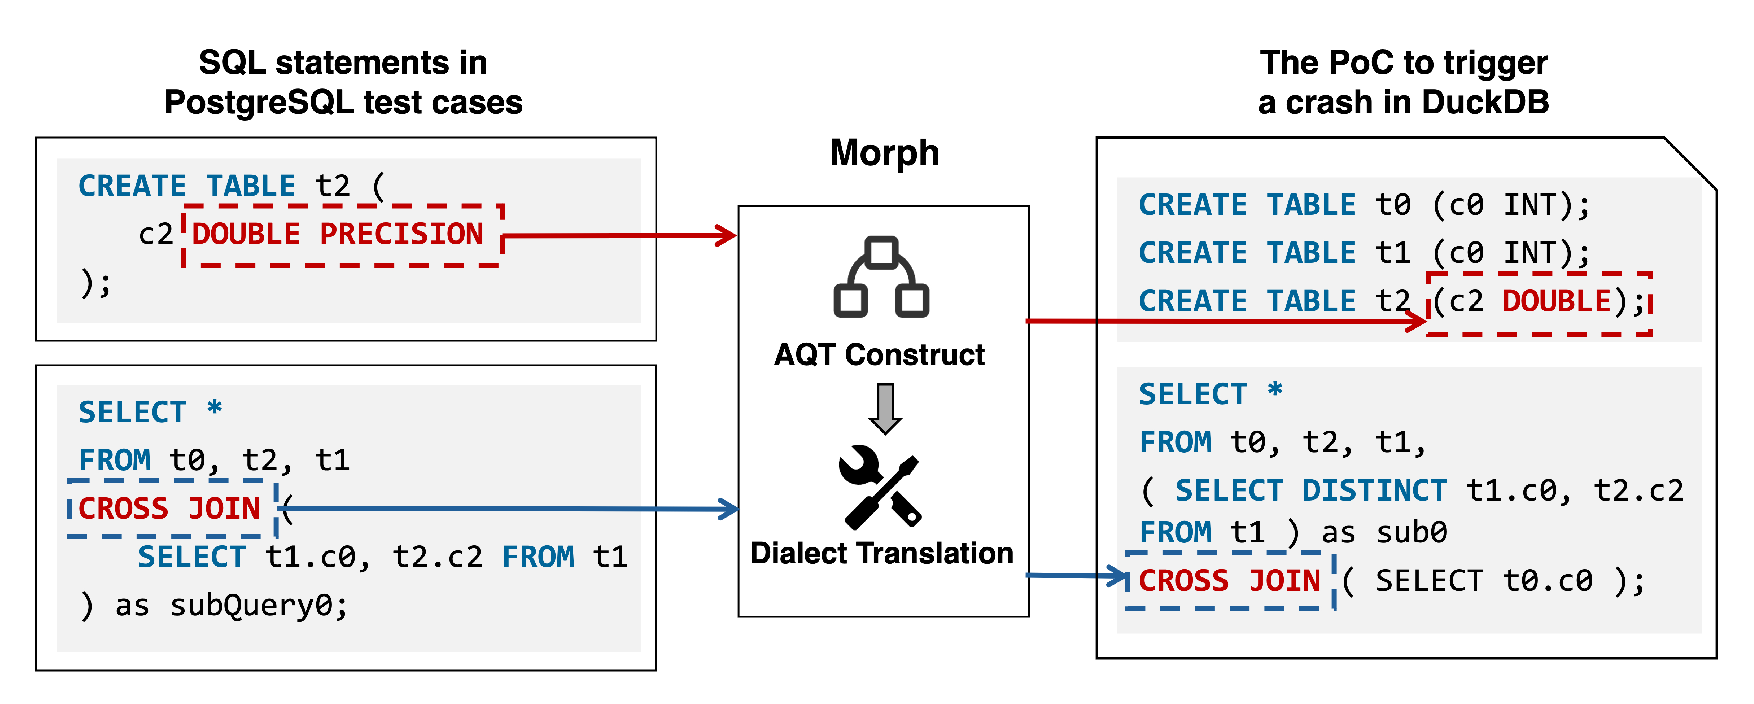
\includegraphics[width=0.8\linewidth]{media/casestudy.pdf}
  \caption{A internel error found in \duckdb{}( Bug \#205xx). \tool{} translates a  test case of \pg{} to \duckdb{} while preserving critical data types and join logic (Left: source query; Right: instantiated query).
  % (Left) Source PostgreSQL query with mixed types. 
  % (Right) The instantiated DuckDB query that successfully triggers a deep executor bug.
  }
  \label{fig:casestudy}
\end{figure}

\tool{}’s effectiveness arises from three key capabilities working in concert, and this bug demonstrates the advantage of its structure-aware transfer. In PostgreSQL, nested joins involving a table with \texttt{DOUBLE PRECISION} joined against a subquery are thoroughly tested, but DuckDB lacks exhaustive coverage for this combination. Traditional migration tools often simplify schemas (e.g., converting \texttt{DOUBLE} to \texttt{INT}) or flatten nested queries to ensure compatibility, which sacrifices semantic precision. By preserving the full complexity of the original seed, \tool{} forced DuckDB to perform detailed type inference and vector allocation for correlated joins, exercising a code path that simplified queries never reach. This high-fidelity transfer uncovered a critical executor logic flaw that had remained undetected precisely because conventional approaches eliminate the structural complexity required to trigger it.

% \tool{}'s success stems from three key capabilities working in concert. This bug exemplifies the unique strength of \tool{}'s structure-aware transfer approach.\duckdb{} lacks exhaustive testing of specific nested join patterns combined with certain data types, whereas \pg{} has rigorous test suites for these features. The source \pg{} test case defines a table with \texttt{DOUBLE PRECISION} and performs a join against a subquery—a combination that appears standard but hides a latent executor vulnerability in \duckdb{}. This stands in sharp contrast to traditional migration tools, which often sacrifice semantic precision for compatibility by simplifying schemas (e.g., converting \texttt{DOUBLE} to \texttt{INT}) or flattening nested structures. By preserving the full complexity of the original seed, \tool{} forced the \duckdb{} engine to perform intricate type inference and vector allocation for correlated joins—a code path that simplified queries never exercise. This high-fidelity transfer exposed a critical logic flaw in the \textit{Executor} that had evaded detection precisely because conventional testing approaches systematically eliminate the structural complexity necessary to trigger it.

% \textit{The Process of Finding the Bug by \tool{}.} This bug exemplifies the unique strength of \tool{}'s structure-aware transfer approach.\duckdb{} lacks exhaustive testing of specific nested join patterns combined with certain data types, whereas \pg{} has rigorous test suites for these features. The source \pg{} test case defines a table with \texttt{DOUBLE PRECISION} and performs a join against a subquery—a combination that appears standard but hides a latent executor vulnerability in \duckdb{}.

% As illustrated in the Morph pipeline, \tool{} first performs \textit{Boundary Detection} and \textit{AQT Generation} to decompose the query into a structure-aware representation. 
% It then utilizes an Adaptive Query Sanitizer to remove syntactic redundancies, such as excess parentheses, ensuring the query is a ``Mutable Seed''. 
% By transferring the \pg{} logic into valid \duckdb{} grammar and maintaining the structural depth of the original test case, Morph succeeded in triggering the crash.
% While traditional migration tools often simplify schemas involving mixed numeric types (e.g., converting \texttt{DOUBLE} to \texttt{INT}) to ensure basic compatibility, \tool{} preserved the exact diverse data types and the nested correlation during the transfer. By maintaining the high-fidelity semantic logic of the original seed, \tool{} forced the DuckDB engine to perform complex type inference and vector allocation for correlated joins. This precision exposed a logic flaw in the \textit{Executor} that simplified, ``flattened'' queries could never reach.

% When the target DBMS returns semantic feedback (e.g., "Illegal type" or "Cannot parse expression"), the \textit{Error-Guided Repair} mechanism dynamically adjusts the query—for example, by wrapping columns with appropriate type conversion functions like toDateTime()—to produce a final seed that is semantically executable. 

% involving multiple tables, 
% nested \texttt{CROSS JOIN}s, and subqueries with correlated columns, as shown in Figure~\ref{fig:casestudy}. 
% The source logic was derived from a PostgreSQL test case, which defines a table with mixed numeric types (e.g., \texttt{DOUBLE PRECISION}) and performs a nested join against a subquery.







\begin{answerbox}
\textbf{Answer to RQ1:} 
% \tool{} proves its practical value by detecting \textbf{16} previously unknown bugs across five widely used DBMSs, covering critical components such as the Optimizer, Executor, and Storage Engine.
In real-world evaluations, \tool{} successfully exposed \bugcnt{} unknown vulnerabilities within four widely used DBMS engines, affecting core components including the Optimizer and Storage Engine.
With \bugconfirmcnt{} bugs confirmed and \bugfixcnt{} bugs already fixed by developers, these results substantiate \tool{}’s ability to generate high-quality, impactful test cases that successfully reveal bugs in popular DBMSs.
% Notably, \textbf{2} bugs have already been fixed and \textbf{9} confirmed by developers, demonstrating \tool{}'s ability to generate high-quality, impactful test cases that traditional tools missed.
\end{answerbox}

\subsection{Effectiveness of Translation in \tool{}}
In this section, we evaluate the effectiveness of the translation in \tool{} in two aspects, namely the validity and the diversity of SQL features of the test cases translated by \tool{}.
% and preserve the semantic richness of source test cases.

\textbf{Validity of the Translated Test Cases.}
We analyze the effectiveness of \tool{} in generating syntactically and semantically valid seeds across four target DBMSs. 
As shown in Table~\ref{tab:validity}, raw seeds ($S^-$) exhibit extremely low validity in the target DBMS. 
For instance, the semantic correctness ratio is 10\% on Virtuoso, while the highest achieved is only 28\% on DuckDB. 
This shows that the direct execution of foreign SQL dialects is largely ineffective due to inherent syntax and functional incompatibilities between engines.
Moreover, \tool{} achieves \synatxratio{} higher syntactic correctness, and \translateratio{} higher semantic correctness for transferred seeds than \sedar{} ($S$) on \duckdb{}, \clickhouse{}, \monetdb{}, and \virtuoso{}, respectively.
While the \sedar{} improves syntactic correctness through LLM-based translation, its gain in \textit{semantic correctness} remains markedly limited. On DuckDB, for example, \sedar{} achieves a high syntactic pass rate of 90\%, yet only 37\% of these queries can actually execute without runtime errors. This significant discrepancy is primarily attributed to semantic hallucinations. As illustrated in our running example, although \sedar{} can correctly translate the query structure, it often retains PostgreSQL-specific functions such as \texttt{AGE()}. These constructs are valid to a general-purpose parser but are unsupported by the DuckDB engine, leading to immediate execution failure.
% First, we analyze the semantic validity of the generated seeds. As shown in Table~\ref{tab:validity}, raw seeds ($S^-$) exhibit low transferability, with semantic correctness ratios dropping as low as 9.7\% on Virtuoso. This confirms that direct execution of foreign SQL dialects is ineffective due to syntax incompatibilities.

% ============================================================
% Table 4: Validity Statistics (RQ4) - 跨栏，居中，不拉伸
% ============================================================
\begin{table*}[!htbp]
\centering % <--- 关键：居中对齐
\caption{Comparison of Syntactic Correctness and Semantic Validity. $S^-$, $S$, and $S^+$ denote Raw Seeds, \sedar{}, and \tool{}, respectively.}
\label{tab:validity} % <--- 标签：用于引用
% 移除 resizebox，使用表格自然宽度
\renewcommand\arraystretch{1}
\setlength{\tabcolsep}{3mm}{
    \begin{tabular}{l|ccc|ccc}
        \toprule
        \multirow{2}{*}{\textbf{DBMS}} & \multicolumn{3}{c|}{\textbf{Syntactic Correctness}} & \multicolumn{3}{c}{\textbf{Semantic Correctness}} \\
         & $S^-$ & $S$ & $S^+$ (vs S) & $S^-$ & $S$ & $S^+$ (vs S) \\ \midrule
        MonetDB & 0.589 & 0.781 & \textbf{0.929} (+19\%) & 0.236 & 0.388 & \textbf{0.776} (+100\%) \\
        Virtuoso & 0.324 & 0.562 & \textbf{0.670} (+19\%) & 0.097 & 0.169 & \textbf{0.629} (+272\%) \\
        DuckDB & 0.674 & 0.895 & \textbf{0.939} (+5\%) & 0.284 & 0.365 & \textbf{0.748} (+105\%) \\
        ClickHouse & 0.613 & 0.821 & \textbf{0.895} (+9\%) & 0.182 & 0.315 & \textbf{0.694} (+120\%) \\ \bottomrule
    \end{tabular}
}
\end{table*}

In contrast, \tool{} ($S^+$) substantially outperforms both baselines across all evaluated systems. On Virtuoso, it achieves a semantic correctness of 63\%, which represents a 272\% improvement over \sedar{}. Consistently, on MonetDB, the semantic correctness reaches 78\%, effectively doubling the performance of \sedar{} with a 100\% increase. Even on DuckDB, where \sedar{} performs relatively better, \tool{} still provides a 105\% boost in semantic validity. 
The empirical data suggests that the \textit{Abstraction-then-Instantiation} paradigm successfully bridges the gap between parsability and execution by mapping logical intent to target constraints. Consequently, \tool{} provides the DBMS fuzzing with seeds that are mostly executable, serving as a viable foundation for testing.


\textbf{SQL features Diversity of the Translated Test Cases.}
Beyond validity, we assessed whether the transferred seeds retain the testing value of the source test cases by analyzing the diversity of valid SQL features across three dimensions: functions, data types, and keywords. 
As summarized in Table~\ref{tab:diversity}, \tool{} demonstrates a consistent ability to maintain a higher degree of structural richness compared to both the raw seeds ($S^-$) and \sedar{} ($S$). 
In aggregate, \tool{} successfully preserves 1,036 distinct functions, 180 unique data types, and 1,368 keywords across the four target DBMSs. 
In contrast, \sedar{} ($S$) only retains 625 functions, 146 data types, and 872 keywords. 
In other words, compared to \sedar, \tool{} covers 633 more functions, 65 more data types, and 616 more keywords.
% the translates to a substantial net increment of +633 functions, +65 data types, and +616 keywords over the raw baseline.

% Beyond validity, we assessed whether the transferred seeds retain the testing value of the source test cases by analyzing the diversity of valid SQL features (functions, data types, and keywords). Table~\ref{tab:diversity} presents the statistics.

% ============================================================
% table3：跨栏但不拉伸 (table* + \centering)
% ============================================================
\begin{table*}[!htbp]
\centering % <--- 让表格居中
\small     % <--- 主动缩小字号，而不是被拉伸
\caption{Statistics of valid SQL features (Functions, Data Types, Keywords) in the transferred seeds.}
\label{tab:diversity}
% 此时不需要 \resizebox，直接放 tabular
\renewcommand\arraystretch{1}
\setlength{\tabcolsep}{3mm}{
    \begin{tabular}{l|ccc|ccc|ccc}
    \toprule
    \multirow{2}{*}{\textbf{DBMS}} & \multicolumn{3}{c|}{\textbf{Functions}} & \multicolumn{3}{c|}{\textbf{Data Types}} & \multicolumn{3}{c}{\textbf{Keywords}} \\
     & $S^-$ & $S$ & $S^+$ & $S^-$ & $S$ & $S^+$ & $S^-$ & $S$ & $S^+$ \\ \midrule
    MonetDB & 107 & 132 & \textbf{161} & 29 & 29 & \textbf{29} & 235 & 244 & \textbf{370} \\
    Virtuoso & 28 & 52 & \textbf{87} & 16 & 17 & \textbf{24} & 102 & 136 & \textbf{335} \\
    DuckDB & 185 & 214 & \textbf{456} & 34 & 39 & \textbf{63} & 291 & 340 & \textbf{476} \\
    ClickHouse & 83 & 227 & \textbf{332} & 36 & 61 & \textbf{64} & 124 & 152 & \textbf{187} \\ \midrule
    \textbf{Total} & 403 & 625 & \textbf{1036} & 115 & 146 & \textbf{180} & 752 & 872 & \textbf{1368} \\
    \textit{Increment} & - & \textit{+222} & \textit{\textbf{+633}} & - & \textit{+31} & \textit{\textbf{+65}} & - & \textit{+120} & \textit{\textbf{+616}} \\ \bottomrule
    \end{tabular}
}
\end{table*}

The improvement in feature diversity is particularly pronounced in engines with significant dialectal gaps, such as DuckDB and Virtuoso. In DuckDB, \tool{} successfully transfers 456 functions, 63 data types, and 476 keywords, effectively doubling the variety across all categories compared to \sedar{}, which only preserves 214 functions, 39 data types, and 340 keywords. A similar trend is observed in Virtuoso, where \tool{} expands the set of valid keywords from 136 to 335 and data types from 17 to 24. These results indicate that \tool{}'s structure-aware approach is more resilient to ``dialect noise'', which frequently causes traditional tools to fail or over-simplify queries. 
By successfully navigating these dialectal disparities, \tool{} retains the intricate functional and type-related details of the source test cases, providing the downstream fuzzer with the diverse inputs required to explore deep execution paths.

The performance gap in diversity primarily originates from the underlying sanitization strategies. \sedar{}~\cite{fu2024sedar} employs a destructive "comment-out" strategy for unparsable tokens, which frequently results in the removal of complex type casts or specialized function calls (e.g., PostgreSQL’s 
% \texttt{::INTERVAL} or 
window function signatures) when they fail to parse in the target engine. Conversely, \tool{} utilizes a constructive paradigm that recursively instantiates these abstract structures into target-compliant forms. For instance, rather than deleting an incompatible interval expression, \tool{} transforms it into the equivalent functional syntax required by DuckDB. Consequently, \tool{} preserves a much broader range of unique data types and functional expressions, ensuring that the downstream fuzzer can explore more diverse type-related execution paths and deeper optimizer logic.
% that typically triggers early rejection or logic loss in traditional translation-based tools.
% \tool{} exhibits a superior capability to preserve structural richness. In terms of functions, \tool{} covers a total of \textbf{1,036} distinct functions across four DBMSs, compared to 625 for \sedar{}. This represents a net increment of +633 valid functions over the raw baseline. A notable improvement is also seen in DuckDB, where \tool{} successfully transfers 456 unique functions and 476 keywords, significantly higher than \sedar{}'s 214 functions and 340 keywords.



% This advantage stems from the difference in sanitization strategies. \sedar{}~\cite{fu2024sedar} employs a destructive strategy (commenting out unparsable tokens), which often removes complex clauses like \texttt{::INTERVAL} when they fail to parse. In contrast, \tool{} recursively instantiates these structures into target-compliant forms (e.g., converting PostgreSQL's interval syntax to DuckDB's standard). Consequently, \tool{} preserves \textbf{180} unique data types across all targets, whereas \sedar{} only retains 146, ensuring that the fuzzer is exposed to a broader range of type-related execution paths.

\begin{answerbox}
\textbf{Answer to RQ2:} \tool{} significantly outperforms baselines in both validity and diversity. It achieves up to 272\% improvement in semantic correctness over \sedar{} and covers 1,036 distinct functions (+633 increment). By eliminating semantic hallucinations and employing constructive instantiation, \tool{} ensures generated seeds are both executable and rich in testing logic.
\end{answerbox}

\subsection{Effectiveness of \tool{} in Improving Fuzzing}
% Beyond the generation phase, we further evaluated the contribution of the \textit{Feedback-Driven Adaptive Sanitizer}. We compared the full framework ($\textsc{Morph}_{\textit{full}}$) against a variant named $\textsc{Morph}_{\textit{static}}$, where the runtime feedback loop is disabled. In the static variant, generated seeds are fed directly to the fuzzer without adaptive repair; if they fail parsing, they are simply discarded.

To evaluate the effectiveness of \tool{} in improving DBMS fuzzing, we compared three different sets of initial seeds. Specifically, $S^-$ denotes directly using the original test cases from the source DBMS as initial seeds; $S$ represents seeds translated by \sedar{} and then fuzzed using the backend fuzzer \griffin{}; and $S^+$ corresponds to seeds translated by \tool{} and fuzzed with \griffin{}. All three configurations were executed under identical experimental settings for 24 hours to ensure a fair comparison.
After the fuzzing campaigns were completed, we conducted a unified dry run of all generated test cases to normalize coverage measurement and eliminate runtime variability. Branch coverage was then collected to quantify testing depth. In addition, we deduplicated crashes using stack trace hashing combined with manual inspection to determine the number of unique bugs discovered by each configuration.

% Based on this setup, we use branch coverage to measure testing depth and the number of unique bugs to evaluate practical effectiveness. As shown in Table~\ref{tab:coverage}, \tool{} ($S^+$) consistently achieves the best performance across all metrics.
% We utilize Branch Coverage to measure the \textit{testing depth} and quantify Unique Bugs to assess the \textit{practical effectiveness} of our approach. 
As illustrated in Table~\ref{tab:coverage}, \tool{} ($S^+$) covers a total of 56\% and 14\% more branches than \sedar{} ($S$) and raw seeds ($S^-$) on four DBMSs, respectively. 
% consistently achieves the highest performance across all metrics.
On embedded OLAP systems like DuckDB, \tool{} covers 144,822 branches, surpassing the raw baseline by 50\% and \sedar{} by 26\%. 
A similar trend is observed in distributed systems; on \clickhouse{}, \tool{} reaches 155,639 branches, an improvement of 78\% over raw seeds. 
Crucially, this deep code penetration directly translates into superior bug discovery capability. As shown in the rightmost columns of Table~\ref{tab:coverage}, \tool{} exposes significantly more unique bugs than baselines. 
Moreover, as shown in Table~\ref{tab:coverage}, \tool{} ($S^+$) detects a total of 12 and 9 more bugs than \sedar{} ($S$) and raw seeds ($S^{-}$) on four DBMSs, respectively. 
% Notably, on MonetDB and DuckDB, \tool{} detected 5 and 4 unique bugs, respectively, whereas \sedar{} only found 1 in each. 
% In total, \tool{} discovered 13 unique bugs across all targets, compared to just 5 by \sedar{}. 
This proves that coverage gains are not merely statistical but functionally impactful, enabling the detection of vulnerabilities that remain unreachable to baselines.

The correlation between semantic validity, coverage, and bug discovery is evident. In the raw baseline ($S^-$), queries often terminate early during parsing due to syntax errors. By ensuring high semantic validity (RQ2), \tool{} allows the fuzzer to bypass early rejection checks, exercise deeper logic within the optimizer and executor, and ultimately trigger more critical vulnerabilities.

% ============================================================
% Branch Coverage & Bugs (RQ3) - 跨栏，居中
% ============================================================
\begin{table*}[!htbp]
\centering
\caption{Comparison of Covered Branch and Detected Bugs (24h). $S^-$, $S$, and $S^+$ denote Raw Seeds, \sedar{}, and \tool{}. Percentages in 4th column indicates coverage improvement over $S$.}
\label{tab:coverage}
\renewcommand\arraystretch{1}
\setlength{\tabcolsep}{3mm}{
    \begin{tabular}{l|ccc|ccc} % l|ccc|ccc 表示左对齐 | 3列居中 | 3列居中
        \toprule
        
        \multirow{2}{*}{DBMS} & \multicolumn{3}{c|}{Covered Branches} & \multicolumn{3}{c}{Detected Bugs} \\
         & $S^-$ & $S$ & $S^+$ (vs $S$) & $S^-$ & $S$ & $S^+$ \\ \midrule
        MonetDB    & 61,981 & 76,142  & \textbf{81,486} (+7\%)  & 0 & 1 & \textbf{6} \\
        Virtuoso   & 24,017 & 36,583  & \textbf{40,183} (+10\%) & 0 & 2 & \textbf{2} \\
        DuckDB     & 96,513 & 114,876 & \textbf{144,822} (+26\%)& 2 & 1 & \textbf{4} \\
        ClickHouse & 87,389 & 141,215 & \textbf{155,639} (+10\%)& 0 & 1 & \textbf{2} \\ 
        \midrule
        Total      & 269,900 & 368,816 & \textbf{422,130} & 2 & 5 & \textbf{14} \\ 
        Improvement & +56\% & +14\% & - & +12 & +9 & - \\      \bottomrule
    \end{tabular}
}
\end{table*}

\begin{answerbox}
\textbf{Answer to RQ3:} \tool{} achieves the highest branch coverage across all target DBMSs. Notably, it surpasses the raw baseline coverage by up to 78\% (on ClickHouse) and \sedar{} by 26\% (on DuckDB). 
This coverage improvement allows \tool{} to discover 12 and 9 more bugs than raw seeds and the state-of-the-art tool \sedar{}, respectively, demonstrating its effectiveness in enhancing DBMS fuzzing and exploring deeper state spaces to uncover bugs.
\end{answerbox}

\subsection{Contribution of Individual Components}
To analyze the specific contributions of the individual components within \tool{}, we conducted an ablation study across two phases. For the \textit{translation phase}, we evaluated four variants using the PostgreSQL-to-DuckDB transfer task:
(1) $\tool{}_{\textit{base}}$: the baseline using direct LLM translation without our core components;
(2) $\tool{}_{\textit{abs}}$: equipped solely with \textit{Syntax-Aware Query Abstraction};
(3) $\tool{}_{\textit{rag}}$: equipped solely with the \textit{Rule-Guided RAG Agent}; and
(4) $\tool{}_{\textit{full}}$: the complete framework integrating both components.

For the \textit{fuzzing phase}, since the \textit{Feedback-Driven Adaptive Sanitizer} operates independently during runtime fuzzing and does not affect translation quality, we further introduce $\tool{}_{\textit{static}}$ as a controlled variant where the runtime feedback loop is disabled and invalid seeds are directly discarded, and compare it against $\tool{}_{\textit{full}}$ where the sanitizer actively repairs parsing errors to maximize seed acceptance.
% The results are summarized in Figure~\ref{fig:ablation_analysis}.

\begin{figure}[h]
  \centering
  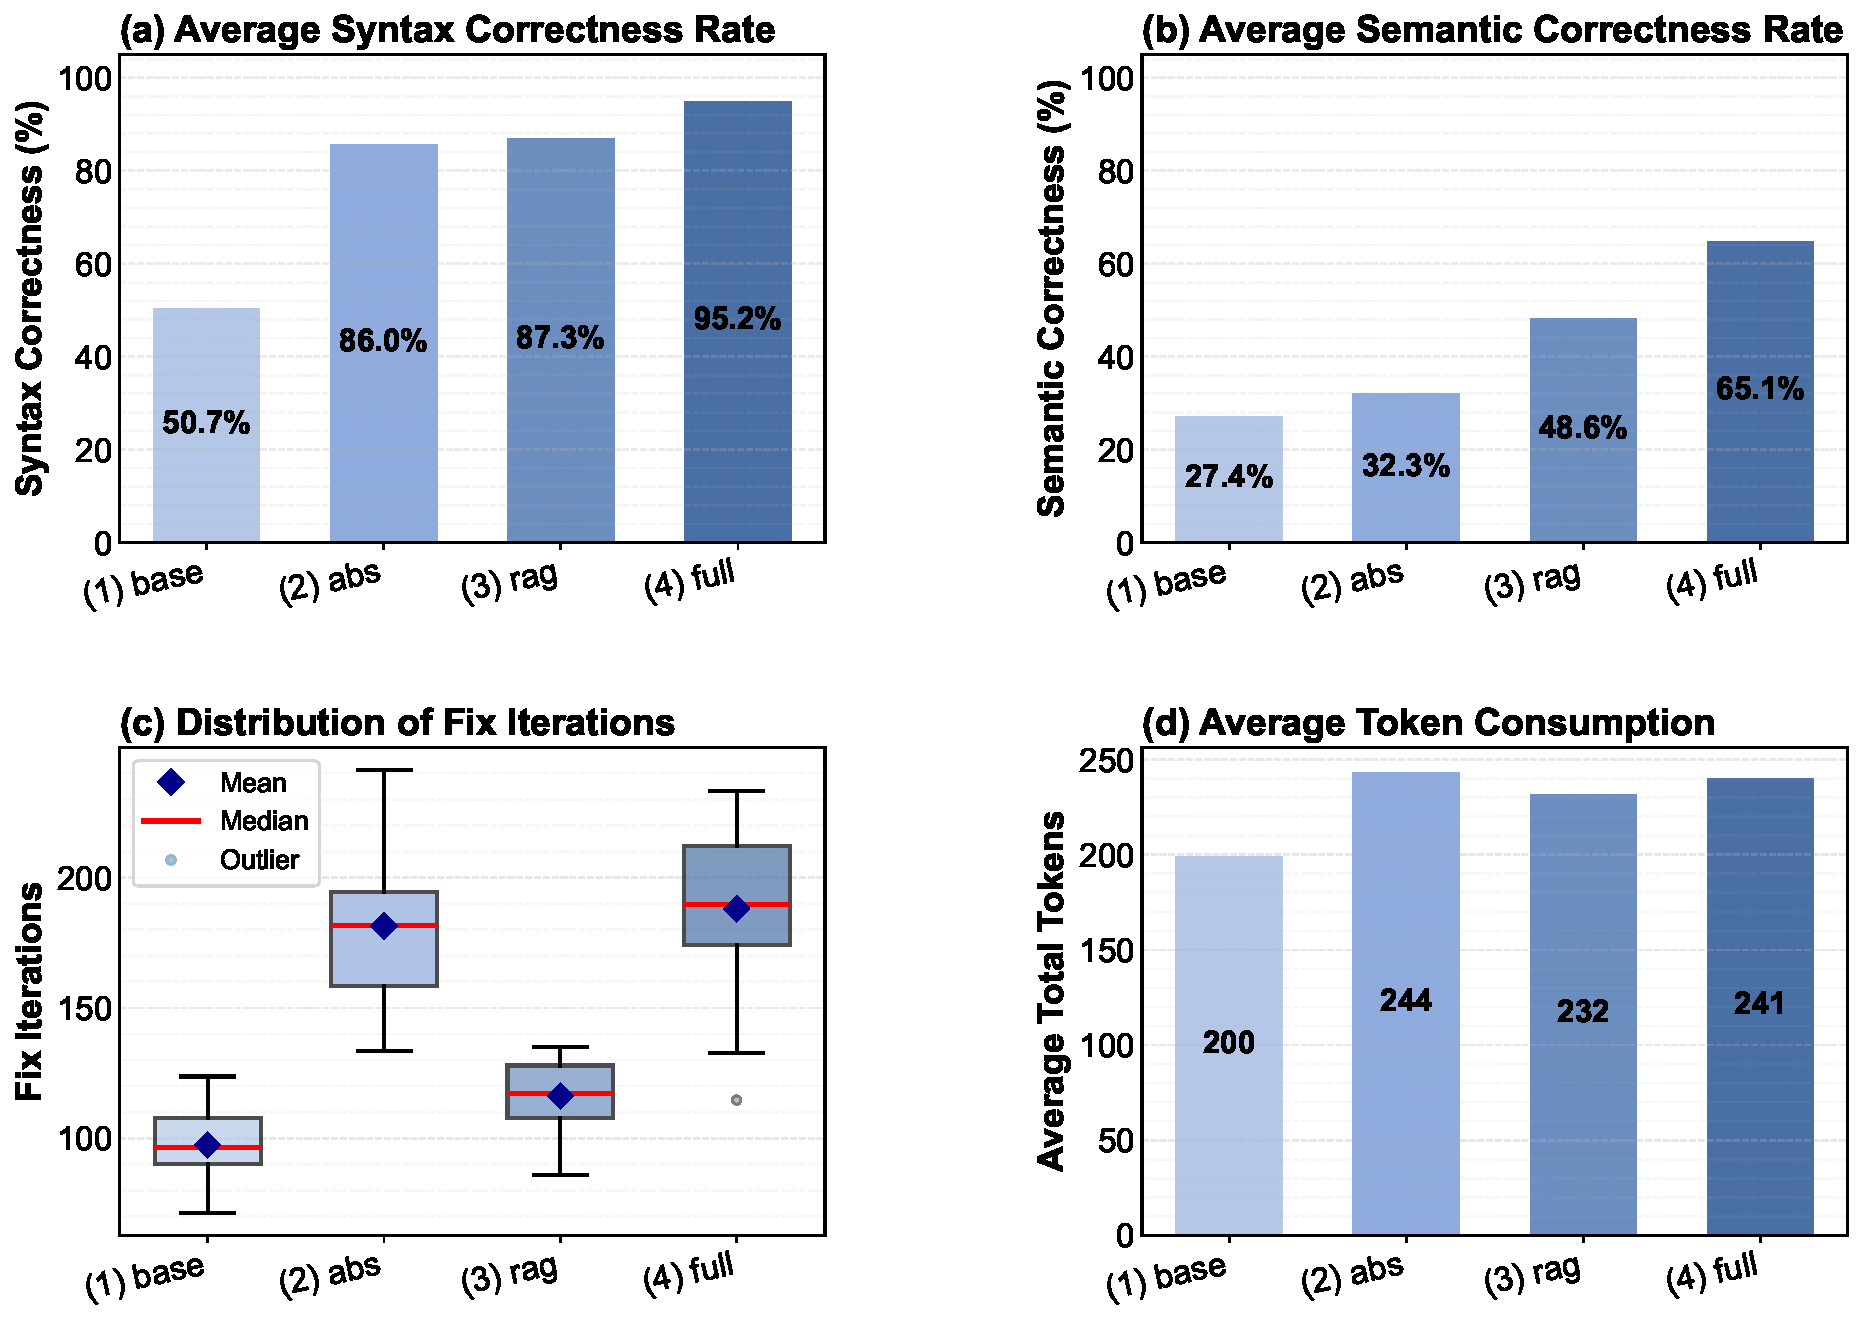
\includegraphics[width=\linewidth]{media/ablation_combined_analysis.pdf}
  \caption{\textbf{Ablation Analysis of \tool{} Components.} Comparison of syntactic/semantic correctness and resource consumption across four variants.}
  \label{fig:ablation_analysis}
\end{figure}

\textbf{Contribution of Syntax-Aware Query Abstraction and Rule-Guided RAG Agent. }
%As illustrated in Figure~\ref{fig:ablation_analysis}, 同时关闭\textit{Syntax-Aware Query Abstraction} and \textit{Rule-Guided RAG Agent}， 语法正确率为50.7%，语义正确率为27.4%。
% 关闭组件\textit{Syntax-Aware Query Abstraction}，语法正确率为50.7%，语义正确率为27.4%
As shown in Figure~\ref{fig:ablation_analysis} (a) and (b), when both the \textit{Syntax-Aware Query Abstraction} and the \textit{Rule-Guided RAG Agent} are disabled, the syntactic correctness is 51\% and the semantic correctness of $\tool{}_{\textit{base}}$ is 27\%.
With \textit{Syntax-Aware Query Abstraction}, $\tool{}_{\textit{abs}}$ improves syntactic correctness to 86\% (+35\%) by leveraging AQT to provide a more stable structural skeleton. The semantic correctness also increases to 32\%.
Moreover, with \textit{Rule-Guided RAG Agent}, $\tool{}_{\textit{rag}}$ further enhances syntax correctness to 87\%, and it also increases correctness to 49\% (+21\%) by grounding generation in retrieved dialect rules.
The Full framework $\tool{}_{\textit{full}}$ achieves the optimal balance, reaching \textbf{95\%} syntactic and \textbf{65\%} semantic correctness.
% $\tool{}_{\textit{base}}$ yields syntactic and semantic correctness of only 50.7\% and 27.4\%, respectively (Figure~\ref{fig:ablation_analysis}(c) and (d)). 

% , albeit with a 16.2\% increase in token consumption (Figure~\ref{fig:ablation_analysis}(f)). 
Figure~\ref{fig:ablation_analysis} (c), (d), (e), and (f) show the data about fix iterations and token consumptions.
While $\tool{}_{\textit{full}}$ introduces a higher iteration cost (+89\%) and token consumption (+21\%) compared to the baseline, these costs are a justified investment for the substantial gain in high-fidelity transfer. 
This confirms that the synergy between the structural guidance of AQT and the semantic constraints of the RAG Agent is essential for improving syntax and semantic correctness.
% discovering bugs.

\begin{table}[b]
\centering
\small
\caption{Ablation study of the Feedback-Driven Sanitizer on Branch Coverage across DBMSs (24h).}
\label{tab:ablation_sanitizer}
\begin{tabular}{lccc}
\toprule
\textbf{DBMS} & \tooldisfuzzer{} & $\tool{}_{\textit{full}}$ & \textbf{Improvement} \\
\midrule
MonetDB    & 67,620 & \textbf{81,486}  & \textbf{+21\%} \\
Virtuoso   & 37,213 & \textbf{40,183}  & \textbf{+8\%} \\
DuckDB     & 118,453 & \textbf{144,822} & \textbf{+22\%} \\
ClickHouse & 112,083 & \textbf{155,639} & \textbf{+39\%} \\
\bottomrule
\end{tabular}
\end{table}

\textbf{Contribution of Feedback-Driven Adaptive Sanitizer.}
% Beyond the generation phase, we further evaluated the contribution of the \textit{Feedback-Driven Adaptive Sanitizer}. 
To evaluate the contribution of the component, we compared the full framework ($\tool{}_{\textit{full}}$) against a variant named \tooldisfuzzer{}, where the runtime feedback loop is disabled. In the static variant, generated seeds are fed directly to the fuzzer without adaptive repair; if they fail parsing, they are simply discarded.
Table~\ref{tab:ablation_sanitizer} presents \tool{} covers 8\% to 39\% more branches across four DBMSs than \tooldisfuzzer{} over a 24-hour campaign. 
% Taking \duckdb{} as an example, \tooldisfuzzer{} achieves a coverage of 118,453 branches. 
When the component is disabled, \tooldisfuzzer{} experiences a high rejection rate by the fuzzer at the parser stage due to syntax mismatches.
In contrast, by actively repairing these specific errors, $\tool{}_{\textit{full}}$ recovers these invalid seeds, allowing them to pass the frontend and are used for fuzzers to explore more state sapce of the target DBMSs. 
% This results in a coverage increase to \textbf{144,822} branches (\textbf{+22.3\%}). 
% This experiment confirms that high-quality generation alone is insufficient; the adaptive sanitization bridge is indispensable for translating ``valid intent'' into ``covered paths.''

\begin{answerbox}
\textbf{Answer to RQ4:} All three components are critical for \tool{}. $\tool{}_{\textit{abs}}$ stabilizes the structural skeleton, improving syntactic correctness by 37\%. $\tool{}_{\textit{rag}}$ ensures semantic alignment, boosting validity by 21\%. $\tool{}_{\textit{full}}$ achieves a cumulative improvement of \textbf{44\%} in syntax and \textbf{38\%} in semantics. 
Furthermore, the \textit{Feedback-Driven Sanitizer} is indispensable for execution depth, boosting branch coverage by up to \textbf{39\%} (on ClickHouse) compared to static generation.
\end{answerbox}


\section{Discussion}
\label{sec:discussion}

% \textbf{Usefulness and Extensibility. }
% We first address the inherent design constraints of \tool{} to clarify its practical utility and scalability. The framework faces two primary challenges: the high computational \textit{overhead} introduced by static analysis and LLM inference, and the \textit{dependency} on source seed richness due to the transfer-based paradigm. 
% To resolve the overhead issue, we frame it as a strategic \textit{one-time offline investment}: by ensuring high semantic correctness offline, we maximize the online \textit{effective execution rate}, thus reducing the amortized cost. Furthermore, a Producer-Consumer architecture allows for high-concurrency generation, effectively hiding inference latency. 
% Regarding dependency, we leverage a \textbf{Data-Driven Scalability} approach. Unlike rule-based tools that require manual maintenance, \tool{} adopts a \textit{Data-as-Rules} design, where extensibility is achieved linearly by ingesting diverse open-source test cases (e.g., from other DBMSs) without modifying the core code.

\textbf{Threats to Validity. }
Finally, we consider potential threats to the validity of our evaluation. \textit{Internal validity} is primarily threatened by the inherent randomness of fuzzing campaigns and the non-determinism of LLM outputs. 
We mitigated this by repeating all experiments 5 times over 24-hour periods and enforcing fixed generation parameters (e.g., temperature) with retrieval constraints to ensure reproducibility. 
\textit{External validity} concerns the generalizability of our results to other database systems. While we selected four representative DBMSs covering Row-store, Column-store, and Multi-model architectures to minimize this threat, extending our approach to non-relational paradigms (e.g., Graph Databases) remains a necessary direction for future work.

\textbf{LLM Parameter Selection. } \label{sec:llm-params}
To ensure reproducibility, we conducted a sensitivity analysis on the temperature parameter across three values (0.2, 0.5, 0.8). Lower temperatures yielded higher consistency: T=0.2 achieved 95\% translation success rate with 91\% first-attempt stability, outperforming T=0.5 (92\%/78\%) and T=0.8 (85\%/70\%). 
These results indicate that lower temperature settings help the model produce more deterministic outputs while still maintaining semantic correctness. 
Based on this analysis, we adopt T=0.2 for all experiments to balance reliability and flexibility, ensuring that the translated queries remain both valid and reproducible across runs.
% We therefore use T=0.2 for all experiments.

% \textbf{Query Complexity Preservation. }
% While our abstraction-then-instantiation paradigm aims to maintain semantic richness, there is a potential concern that high validity rates might come at the cost of simplified queries. However, our diversity analysis (Table~\ref{tab:diversity}) demonstrates that \tool{} retains significantly more syntax elements (functions, data types, keywords) than baselines, confirming that validity stems from precise structural adaptation.

\textbf{Extend \tool{} to Find Logic Bugs.} 
Beyond test case translation, \tool{} can also be extended to detect logical or semantic bugs. For example, test oracles from tools like SQLancer~\cite{sqlancer} can be migrated across SQL dialects, and result discrepancies can reveal correctness issues. Similarly, semantically equivalent queries can be executed on different DBMSs, with differences highlighting subtle bugs. These extensions leverage \tool{}’s structure-aware translation and adaptive sanitization to uncover a broader range of DBMS errors. In addition, \tool{}’s abstraction and mutation mechanisms can be combined with differential testing or cross-engine consistency checks, enabling systematic exploration of corner cases that are difficult to reach with traditional fuzzing. By preserving both logical intent and structural complexity, \tool{} can expose subtle type inference errors, optimizer misbehaviors, or semantic deviations that would otherwise remain undetected.

% Beyond test case translation, \tool{} can also be extended to detect logical or semantic bugs. For example, test oracles from tools like SQLancer~\cite{sqlancer} can be migrated across SQL dialects, and result discrepancies can reveal correctness issues. Similarly, semantically equivalent queries can be executed on different DBMSs, with differences highlighting subtle bugs. These extensions leverage \tool{}’s structure-aware translation and adaptive sanitization to uncover a broader range of DBMS errors.
% In addition, \tool{}’s abstraction and mutation mechanisms can be combined with differential testing or cross-engine consistency checks, enabling systematic exploration of corner cases that are difficult to reach with traditional fuzzing.

% We acknowledge two inherent limitations of our approach. 
% Second, crash frequency trade-off: \tool{} may trigger fewer raw parser crashes compared to baselines like \sedar{}~\cite{fu2024sedar}. This reflects a deliberate design choice prioritizing depth over frequency. By ensuring seeds pass frontend parsing checks, \tool{} focuses testing effort on deeper components (Optimizer, Executor, Storage Engine), where bugs are scarcer but typically more impactful.



%  直接描述
% \begin{figure}[h]
%   \centering
%   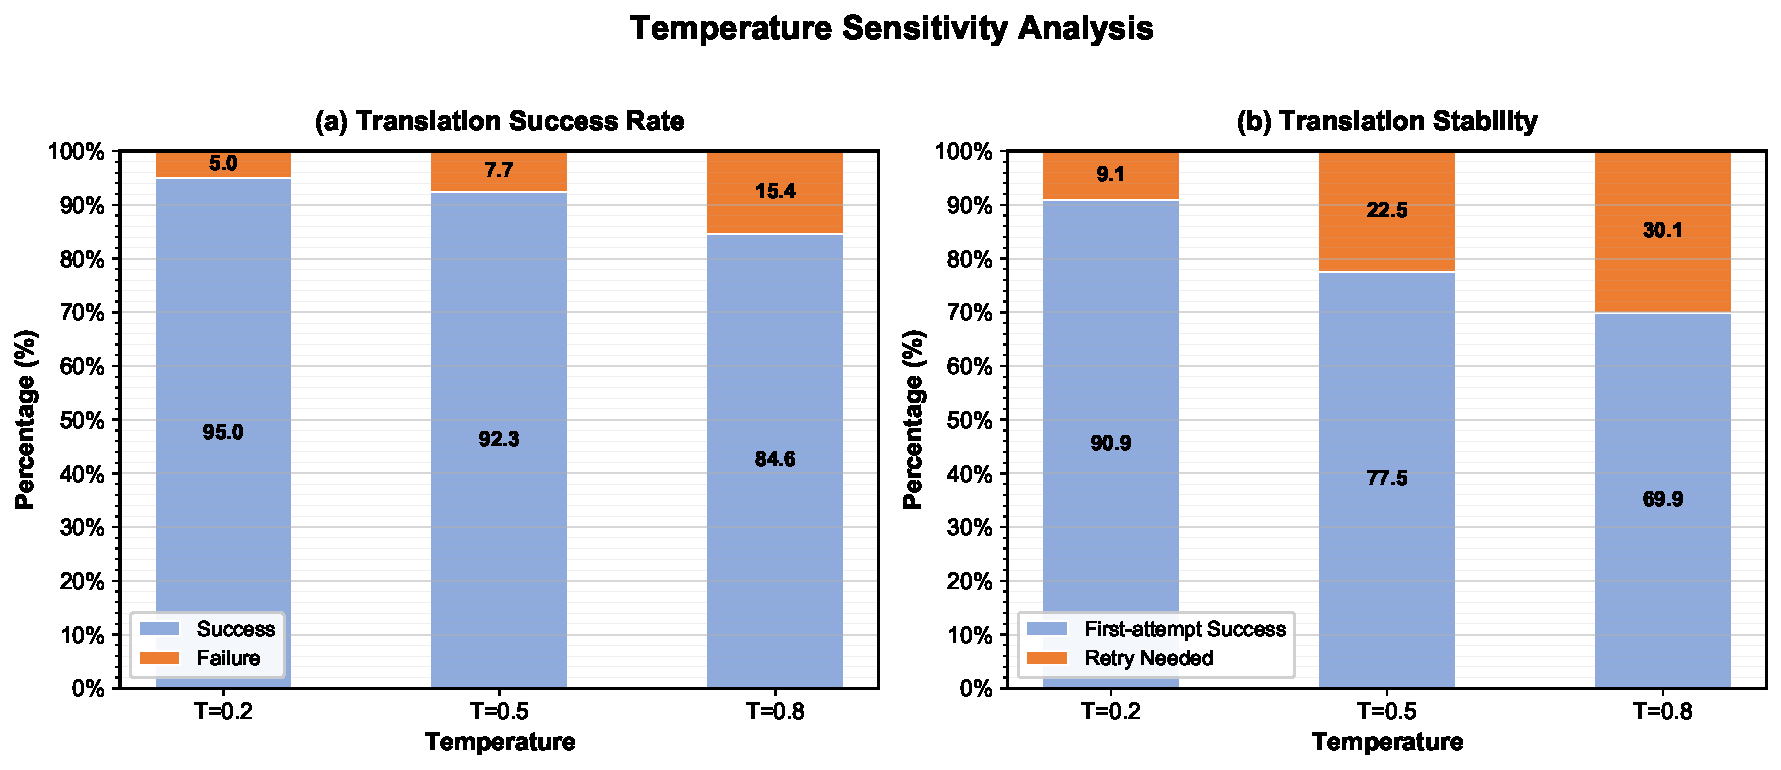
\includegraphics[width=0.7\linewidth]{media/temperature_comparison_simple.pdf}
%   \caption{\textbf{LLM Temperature Sensitivity Analysis.} Comparison of translation success rate and output stability across different temperature settings (T=0.2, 0.5, 0.8). Lower temperature yields higher consistency and success rates.}
%   \Description{A bar chart showing LLM temperature sensitivity analysis with three temperature values (0.2, 0.5, 0.8) comparing translation success rate and output stability metrics.}
%   \label{fig:temperature-sensitivity}
% \end{figure}



\section{Related Work}
\label{sec:related_work}

% We position \tool{} within the broader landscape of DBMS fuzzing and SQL generation, distinguishing it from traditional techniques and recent LLM-based approaches.

\subsection{DBMS Fuzzing}
Fuzzing is one of the most effective automated testing techniques for identifying DBMS vulnerabilities.
% ~\cite{rigger2020detecting, rigger2020finding}. 
Generally, current DBMS fuzzers are categorized into generation-based and mutation-based approaches. Generation-based tools, such as SQLsmith~\cite{sqlsmith}, SQLancer~\cite{sqlancer, rigger2020testing}, and DynSQL~\cite{jiang2023dynsql}, construct SQL queries from scratch using hard-coded rules or semantic oracles. Recent advancements in this category include clause-guided methods~\cite{wei2024sqlaser, ba2023testing}, differential execution~\cite{song2023testing, cui2022differentially}, and specialized frameworks like Pinolo~\cite{hao2023pinolo}. However, these tools are often constrained by predefined templates, which limit their ability to cover complex scenarios~\cite{gao2023comprehensive}. Conversely, mutation-based fuzzers explore deeper code paths by evolving queries from existing seed pools. 
\squirrel{}~\cite{zhong2020squirrel} introduces an intermediate representation (IR) to perform structure-preserving mutations, while \griffin{}~\cite{fu2022griffin} utilizes grammar-free metadata replacement. To further improve code coverage, Lego~\cite{liang2023sequence} proposes sequence-oriented fuzzing by combining different SQL statement sequences, while other works~\cite{yang2024towards} focus on enhancing mutation diversity and reducing grammar dependence. 
% Traditional DBMS fuzzing techniques are generally categorized into generation-based and mutation-based approaches.

% \textbf{Generation-based Fuzzers.} 
% Tools such as SQLsmith~\cite{sqlsmith}, SQLancer~\cite{sqlancer, rigger2020testing}, and DynSQL~\cite{jiang2023dynsql} construct queries from scratch using hard-coded rules or oracle mechanisms (NoREC, TLP~\cite{rigger2020detecting, rigger2020finding}). 
% Recent advances include Pinolo~\cite{hao2023pinolo}, differential execution approaches~\cite{song2023testing, cui2022differentially}, and clause-guided methods~\cite{wei2024sqlaser, ba2023testing}. 
% However, these tools are often constrained by predefined templates, limiting coverage of complex scenarios~\cite{gao2023comprehensive}.
% \textbf{Generation-based Fuzzers.} 
% Tools such as SQLsmith~\cite{sqlsmith}, SQLancer~\cite{sqlancer, rigger2020testing}, and DynSQL~\cite{jiang2023dynsql} construct queries from scratch, relying on hard-coded syntactic rules, stateful generation, or specific oracle mechanisms like NoREC and TLP~\cite{rigger2020detecting, rigger2020finding}. 
% Recent advances include Pinolo~\cite{hao2023pinolo} for approximate query synthesis and differential query execution~\cite{song2023testing, cui2022differentially} for detecting logic bugs across transaction boundaries.
% Recent clause-guided approaches, such as SQLaser~\cite{wei2024sqlaser} and query plan guidance~\cite{ba2023testing}, further model error-prone function chains to detect logic bugs. 
% While these tools excel at detecting logic bugs through rigorous oracle checks or state-aware generation, the queries they generate are often constrained by predefined templates or fixed knowledge, limiting their ability to cover complex, real-world business scenarios~\cite{gao2023comprehensive}.

% \textbf{Mutation-based Fuzzers.} 
% SQUIRREL~\cite{zhong2020squirrel} and GRIFFIN~\cite{fu2022griffin} rely on seed pools: SQUIRREL performs structure-preserving mutations via IR, while GRIFFIN uses grammar-free metadata replacement. 
% Recent efforts~\cite{liang2023sequence, yang2024towards} improve mutation diversity and reduce grammar dependence.


Existing studies primarily focus on the mechanisms of \textit{how to mutate} or \textit{how to detect} bugs, different from them, \tool{} addresses the upstream challenge of \textit{seed acquisition}. As an orthogonal and complementary approach~\cite{zhong2020squirrel, jiang2023dynsql}, \tool{} provides high-quality cross-dialect seeds that unlock the testing potential for complex scenarios and emerging DBMS engines~\cite{gao2023comprehensive}.
% These tools focus on \textit{how to mutate} or \textit{detect bugs}, while \tool{} addresses the upstream challenge of \textit{seed acquisition}. 
% \tool{} is orthogonal and complementary~\cite{zhong2020squirrel, jiang2023dynsql}, providing high-quality cross-dialect seeds to unlock deep testing capabilities, especially for emerging engines~\cite{gao2023comprehensive}.

\subsection{LLM-Based Seeds Generation}
Several recent works integrate LLMs to generate high-quality initial seeds for DBMS testing. CrackSQL~\cite{zhou2025cracking} employs genetic algorithms alongside LLMs to mine complex mutation patterns, while RISE~\cite{xie2026rise} performs rule-driven dialect translation of single SELECT statements via query reduction. Fuzz4All~\cite{xia2024fuzz4all} demonstrates the versatility of LLM prompting for input generation across multiple software domains. While these intra-dialect approaches effectively improve query variety, they are often insufficient for emerging DBMSs due to the scarcity of engine-specific training data. To address this, \sedar{}~\cite{fu2024sedar} introduces end-to-end translation with commenting-out sanitization to facilitate cross-dialect migration, yet it remains susceptible to semantic hallucinations. Recent efforts such as ShQveL~\cite{zhong2025testing} and QTRAN~\cite{lin2025qtran} further focus on fragment synthesis and metamorphic-oracle extensions to improve testing coverage. Despite these advancements, ensuring semantic fidelity across heterogeneous SQL engines remains a persistent challenge.
% Recent advancements have integrated Large Language Models (LLMs) into fuzzing loops to enhance query diversity.
% \textbf{Intra-Dialect Generation and Cross-Dialect Transfer.} In the domain of intra-dialect generation, CrackSQL~\cite{zhou2025cracking} uses genetic algorithms with LLMs to mine mutation patterns, RISE~\cite{xie2026rise} performs rule-driven SELECT dialect translation via query reduction, and Fuzz4All~\cite{xia2024fuzz4all} applies LLM prompting across domains. Extending to cross-dialect transfer, \sedar{}~\cite{fu2024sedar} uses LLM end-to-end translation with commenting-out sanitization, yet it suffers from semantic hallucinations via textual translation. Recent efforts also include ShQveL~\cite{zhong2025testing} for fragment synthesis and QTRAN~\cite{lin2025qtran} for metamorphic-oracle extension; while these improve coverage and extensibility, they inherit cross-dialect fidelity challenges.

% \textit{Relation to \tool{}.} In contrast to intra-dialect approaches that operate within single dialects, \tool{} elevates this to \textit{cross-dialect} transfer via AQT and recursive instantiation, overcoming syntactic and semantic disparities across DBMSs. To address the fidelity issues in existing cross-dialect methods, \tool{} adopts \textit{Abstraction-then-Instantiation} with recursive AST substitution to constrain LLM generation and ensure semantic equivalence. Furthermore, unlike \sedar{}'s destructive sanitization, \tool{}'s \textit{Adaptive Sanitizer} proactively repairs incompatible features, preserving logic required for deep bug detection.

Unlike intra-dialect approaches, \tool{} achieves \textit{cross-dialect} transfer via AQT and recursive instantiation, overcoming DBMS disparities. To address fidelity challenges, \tool{} employs \textit{Abstraction-then-Instantiation} with recursive AST substitution to preserve semantic complexity. Addtionally, \sedar{} relies on destructive sanitization that may compromise query integrity, \tool{}'s Adaptive Sanitizer proactively repairs dialect-specific features to preserve original logic, thereby enabling deeper bug detection in DBMSs.

% \textbf{Intra-Dialect Generation.} 
% CrackSQL~\cite{zhou2025cracking} uses genetic algorithms with LLMs to mine mutation patterns, RISE~\cite{xie2026rise} performs rule-driven SELECT dialect translation via query reduction, and Fuzz4All~\cite{xia2024fuzz4all} applies LLM prompting across domains.


% \textit{Relation to \tool{}:} 
% These approaches operate within single dialects. \tool{} elevates this to \textit{cross-dialect} transfer via AQT and recursive instantiation, overcoming syntactic and semantic disparities across DBMSs.

% \textbf{Cross-Dialect Transfer.} 
% \sedar{}~\cite{fu2024sedar} uses LLM end-to-end translation with commenting-out sanitization. 
% Recent efforts include ShQveL~\cite{zhong2025testing} for fragment synthesis, QTRAN~\cite{lin2025qtran} for metamorphic-oracle extension, and CrackSQL~\cite{zhou2025cracking} for genetic optimization.

% \textit{Relation to \tool{}:} 
% \sedar{}~\cite{fu2024sedar} suffers from semantic hallucinations via textual translation. 
% While ShQveL~\cite{zhong2025testing} and QTRAN~\cite{lin2025qtran} improve coverage and extensibility, they inherit cross-dialect fidelity challenges. 
% \tool{} adopts \textit{Abstraction-then-Instantiation} with recursive AST substitution to constrain LLM generation and ensure semantic equivalence. 
% Unlike \sedar{}'s destructive sanitization, \tool{}'s \textit{Adaptive Sanitizer} proactively repairs incompatible features, preserving logic required for deep bug detection.



\section{Conclusion}
\label{sec:conclusion}
% In this paper, we propose \tool{}, an automated framework designed to bridge the semantic barriers in cross-dialect DBMS fuzzing through structure-aware SQL transfer.
% By establishing the \textit{Abstraction-then-Instantiation} paradigm, \tool{} effectively decouples logical intent from syntactic representation. The system orchestrates a static analysis engine to extract dialect-agnostic AQT, employs a rule-guided RAG agent to recursively instantiate these templates into target dialects, and utilizes an adaptive sanitizer to ensure seamless integration with downstream fuzzers.
% Extensive evaluations across four distinct DBMS architectures demonstrate that \tool{} significantly outperforms state-of-the-art baselines, improving semantic validity by up to \textbf{272\%} and achieving superior code coverage. Furthermore, its practical efficacy is evidenced by the discovery of \bugcnt{} previously unknown bugs, covering critical components from the optimizer to the storage engine.
% Future work will explore extending this structural transfer paradigm to non-relational systems, such as Graph and Time-Series databases, to further broaden the scope of automated database testing.
In this paper, we propose \tool{}, an automated framework designed to bridge semantic gaps in cross-dialect DBMS fuzzing through structure-aware SQL transfer. \tool{} introduces a testing logic abstraction and instantiation workflow that effectively separates logical intent from specific syntax. 
Specifically, the framework first extracts dialect-agnostic AQTs, and then employs a rule-guided RAG agent to instantiate these AQTs for target dialects. 
Finally, it applies an adaptive query sanitizer to ensure compatibility with downstream fuzzers. 
Our evaluations across four DBMSs show that \tool{} outperforms state-of-the-art baseline \sedar{}, improving semantic validity by up to 272\% and achieving superior code coverage. Moreover, \tool{} has successfully detected \bugcnt{} previously unknown bugs in four popular DBMSs, covering critical components from the optimizer to the storage engine. Our future work will explore extending this structural transfer paradigm to non-relational systems, such as Graph and Time-Series databases, to further broaden the scope of automated database testing.

\section{Data Availability}
The source code and experimental data are available at the anonymous repository: \url{https://anonymous.4open.science/r/Morph-82DE}.



\bibliographystyle{ACM-Reference-Format}
\bibliography{bibfile} 


\end{document}
\endinput
%%
%% End of file `sample-acmsmall-submission.tex'.
